%%%%%%%%%%%%%%%%%%%%%%%%%%%%%%%%%%%%%%%%%%%%%%%%%%%%%%%%%%%%%%%%%%%%%%%%%%%%%%%%
%2345678901234567890123456789012345678901234567890123456789012345678901234567890
%        1         2         3         4         5         6         7         8

\documentclass[letterpaper, 10 pt, mydraft, conference]{ieeeconf}  % Comment this line out if you need a4paper

%\documentclass[a4paper, 10pt, conference]{ieeeconf}      % Use this line for a4 paper

\IEEEoverridecommandlockouts                              % This command is only needed if 
                                                          % you want to use the \thanks command

\overrideIEEEmargins                                      % Needed to meet printer requirements.

% See the \addtolength command later in the file to balance the column lengths
% on the last page of the document

% The following packages can be found on http:\\www.ctan.org
%\usepackage{graphics} % for pdf, bitmapped graphics files
%\usepackage{epsfig} % for postscript graphics files
%\usepackage{mathptmx} % assumes new font selection scheme installed
%\usepackage{times} % assumes new font selection scheme installed
%\usepackage{amsmath} % assumes amsmath package installed
%\usepackage{amssymb}  % assumes amsmath package installed

\usepackage[english]{babel}

\usepackage{graphics} 		% for pdf, bitmapped graphics files
\usepackage{graphicx}
\usepackage{epsfig} 		% for postscript graphics files
\usepackage{epstopdf}

\usepackage{listings}
\usepackage{color}
\usepackage{nameref}
\usepackage[bookmarks=true]{hyperref}
\usepackage[colorinlistoftodos]{todonotes}
%\usepackage{index}
%\usepackage{pgfgantt}
\usepackage{amsmath}	 	% assumes amsmath package installed
\usepackage{amssymb}  		% assumes amsmath package installed

\usepackage{dsfont}
\usepackage{mathtools}

\usepackage{epigraph}
\usepackage{lscape}
\usepackage[]{nomencl}		% nomenclatures
\usepackage[ruled,vlined]{algorithm2e}
\usepackage{multicol}
\usepackage{multirow}
\usepackage{etoolbox}

\usepackage{caption}
\usepackage[labelformat=simple]{subcaption}
\renewcommand\thesubfigure{(\alph{subfigure})}
\usepackage{wrapfig}

%\usepackage{flushend}

\usepackage{units}
%\usepackage{flushend}


\pdfminorversion=4

%========================================================
% GENERAL
%--------------------------------------------------------

\renewcommand{\sec}{Section~}
\newcommand{\fig}{Fig.~}
\newcommand{\eq}{}
\newcommand{\app}{Appendix~}
\newcommand{\tab}{Table~}
\newcommand{\alg}{Alg.~}
%\newcommand{\line}{Line~}

\newcommand{\newword}[1]{\textbf{#1}}

%\newindex{todo}{tod}{tnd}{TODO List} % start todo list
%\newindex{fixme}{fix}{fnd}{FIXME List} % start fixme list
%\newcommand{\todo}[1]{\textcolor{blue}{TODO: #1}\index[todo]{#1}} % macro for todo entries
%\newcommand{\fixme}[1]{#1}
%\DeclareOption{mydraft}{\renewcommand{\fixme}[1]{\textcolor{red}{\textbf{#1}}}}
%\ProcessOptions

\newcommand{\fixme}[1]{}
\DeclareOption{mydraft}{\renewcommand{\fixme}[1]{\textcolor{red}{#1}}} 		% macro for fixme entries
\ProcessOptions
\newcommand{\comment}[1]{}
\DeclareOption{mydraft}{\renewcommand{\comment}[1]{\textcolor{blue}{\textbf{[NdR: #1]}}}}		% macro for comment
\ProcessOptions

% Colors used in Matlab plots
\definecolor{matlab1}{rgb}{0,0,1}
\definecolor{matlab2}{rgb}{0,0.5,0}
\definecolor{matlab3}{rgb}{1,0,0}
\definecolor{matlab4}{rgb}{0,0.75,0.75}
\definecolor{matlab5}{rgb}{0.75,0,0.75}
\definecolor{matlab6}{rgb}{0.75,0.75,0}
\definecolor{matlab7}{rgb}{0.25,0.25,0.25}


\definecolor{darkgreen}{rgb}{0,0.5,0}		%Olivegreen?
\definecolor{purple}{rgb}{0.75,0,0.75}
\definecolor{pink}{rgb}{1,0.4,0.6}


\newcommand{\specialcell}[2][c]{%
  \begin{tabular}[#1]{@{}c@{}}#2\end{tabular}}
  
\newcommand{\unknown}[0]{\fixme{XXX}}
\newcommand{\missingcitation}[0]{\fixme{\cite{???}}}

\providecommand{\SetAlgoLined}{\SetLine}
\providecommand{\DontPrintSemicolon}{\dontprintsemicolon}


%========================================================
% MATH
%--------------------------------------------------------

\renewcommand{\vec}{\boldsymbol}				% Vector
\newcommand{\mat}{\boldsymbol}					% Matrix
\DeclareMathOperator{\diag}{\mathrm{diag}} 			% Diagonal matrix

\newcommand{\R}[0]{\mathds{R}}					% Real numbers

\renewcommand{\d}{\mathrm{d}}					% Derivate
\newcommand{\gradient}{\nabla}					% Gradient
\newcommand{\hessian}{H}					% Hessian
\nomenclature{\hessian}{Hessian}

\newcommand{\inv}[0]{^{-1}} 					% Inverse
%\newcommand{\T}[0]{^T} 						% Transpose % \top
\newcommand{\T}[0]{^\top} 						% Transpose % \top

\newcommand{\norm}[1]{\left|\left| #1 \right|\right|} 		% Norm
\newcommand{\asin}[0]{\sin^{-1}} 	% 

\newcommand{\E}{\mathds{E}}	 				% expectation operator
\DeclareMathOperator{\var}{\mathrm{var}} 			% variance
\newcommand{\prob}{{p}} 					% probability density function
\newcommand{\normcdf}[1]{\Phi\left( #1 \right)} 		% Normal Cumulative distribution function
\newcommand{\normpdf}[1]{\phi\left( #1 \right)} 		% Normal probability density function
\newcommand{\gauss}[2]{\mathcal{N} \left( #1,#2 \right)}	% Gaussian Distribution


%========================================================
% MACHINE LEARNING
%--------------------------------------------------------

\newcommand{\dataset}[0]{\mathds{D}} 				% Dataset
\newcommand{\trainingset}[0]{\mathcal{D}}

\newcommand{\inputMatrix}[0]{\mat x}
\newcommand{\inputSpace}[0]{\mathcal{X}}
\newcommand{\outputMatrix}[0]{\mat y}
\newcommand{\regressionNo}[0]{f}

%========================================================
% GAUSSIAN PROCESSES
%--------------------------------------------------------

%\newcommand{\GP}[0]{\text{GP}} % Gaussian process
\newcommand{\GP}[0]{\mathcal{GP}} 	% Gaussian Process
\newcommand{\noise}[0]{w}

%========================================================
% OPTIMIZATION
%--------------------------------------------------------

\DeclareMathOperator*{\argmin}{arg\,min}
\DeclareMathOperator*{\minimize}{\text{minimize}}
\newcommand{\parameters}[0]{\vec x} 			% Parameters
\newcommand{\dimparameters}{d}					% Dimensionality parameters
\newcommand{\iteration}[0]{i}

\newcommand{\objfuncNo}[0]{f}					% Objective function
\newcommand{\objfunc}[1]{\objfuncNo\left(#1\right)}		% Objective function (as a function)
\newcommand{\respsurfNo}[0]{\hat \objfuncNo}			% Response surface
\newcommand{\respsurf}[1]{\respsurfNo \left( #1 \right)} 	% Response surface (as a function)
\newcommand{\acqfuncNo}[0]{\alpha}				% Acquisition function
\newcommand{\acqfunc}[1]{\acqfuncNo \left( #1 \right)}		% Acquisition function (as a function)
\newcommand{\acqsurf}[1]{\acqfuncNo \left( #1 \right)}		% Acquisition surface
\newcommand{\gradientline}{\d \objfunc{\parameters}/\d \parameters}

% Multi-objective optimization
\newcommand{\numbersubobj}[0]{n}
\newcommand{\mergefuncmooNo}[0]{z}
\newcommand{\mergefuncmoo}[1]{\mergefuncmooNo \left( #1 \right)}
\newcommand{\weightsmoo}[0]{\alpha}
\newcommand{\subobjfuncNo}[0]{g}
\newcommand{\subobjfunc}[1]{\subobjfuncNo \left( #1 \right)}


%========================================================
% Neural Networks
%--------------------------------------------------------

\newcommand{\nntf}[1]{\sigma \left( #1 \right)} 		% Neural Networks Transfer function
\newcommand{\nnBh}[0]{\vec {Bh}} 				% Neural Networks Bias of Hidden layer
\newcommand{\nnB}[0]{\vec B} 					% Neural Networks Bias
\newcommand{\nnW}[0]{\mat W} 					% Neural Networks Weights
\newcommand{\nnE}[0]{E} 					% Neural Networks Error function


%========================================================
% ROBOTICS
%--------------------------------------------------------

\newcommand{\q}{\mat q}
\newcommand{\dq}{\dot{\q}}
\newcommand{\ddq}{\ddot{\q}}
\newcommand{\skinInput}{\mathcal{\vec S}}

\newcommand{\frictionMatrixNo}[0]{\mat f}
\newcommand{\inertiaMatrixNo}[0]{\mat M}
\newcommand{\inertiaMatrix}[0]{\inertiaMatrixNo \left( \q \right)}
\newcommand{\gravityMatrixNo}[0]{\vec g}
\newcommand{\torque}{\tau}
\newcommand{\torques}[0]{\vec \torque}
%\newcommand{\forceNo}[0]{\vec F}
\newcommand{\extForce}[0]{\gamma}
\newcommand{\extForces}[0]{\vec \extForce}
\newcommand{\ftsForce}{F}
\newcommand{\ftsForces}{\vec \ftsForce}
\newcommand{\jtsForce}{\tau}%_text{JTS}}
\newcommand{\jtsForces}{\vec \jtsForce}%_text{JTS}}
\newcommand{\Hmatrix}[0]{\vec h \left(\q,\dq \right)}
\newcommand{\jacobian}[0]{\mat J}
\newcommand{\coriolis}[0]{C}

%========================================================
\ProcessOptions
%========================================================

\newcommand{\idyn}[0]{\textit{iDyn}}

\newcommand{\robot}{\textit{iCub}}

\newcommand{\figspace}{\vspace{-10pt}}


\title{\LARGE \bf
%Learning Whole-Body Control with Tactile Sensing
%Learning forward and inverse dynamics of contacts using tactile sensing
%Learning dynamics models of contacts using tactile sensing
%Predicting Joint Torques in Inverse Dynamics Models with Contacts
Learning Inverse Dynamics Models with Contacts
}


\author{Roberto Calandra$^{1}$, Serena Ivaldi$^{1,2}$, Marc Peter Deisenroth$^{3}$, Elmar Rueckert$^{1}$, Jan Peters$^{1,4}$% <-this % stops a space
\thanks{*The research leading to these results has received funding from the European Community's Seventh Framework Programme (FP7/2007--2013) under grant agreements \#270327 (CompLACS) and \#600716 (CoDyCo). MPD has been supported by an Imperial College Junior Research Fellowship.}% <-this % stops a space
\thanks{We thank V. Padois and A. Droniou for their help with \textit{iCubParis02}.}
\thanks{$^{1}$Intelligent Autonomous Systems, TU Darmstadt, Darmstadt, Germany}%
\thanks{$^{2}$Inria, Villers-l\`es-Nancy, F-54600, France; CNRS, Loria, UMR n.7503 and Universit\'e de Lorraine, , Vandoeuvre-l\`es-Nancy, F-54500, France}%
\thanks{$^{3}$Department of Computing, Imperial College London, London, UK}%
\thanks{$^{4}$Max Planck Institute for Intelligent Systems, T\"ubingen, Germany} %
}

\begin{document}



\maketitle
\thispagestyle{empty}
\pagestyle{empty}


%%%%%%%%%%%%%%%%%%%%%%%%%%%%%%%%%%%%%%%%%%%%%%%%%%%%%%%%%%%%%%%%%%%%%%%%%%%%%%%%

\begin{abstract}
	% READ: http://www.ausy.tu-darmstadt.de/HowTo/WritingAnEffectiveAbstract
%
% To deal with contacts in whole-body control it is necessary to estimate 
% accurately joint torques and external forces.
%
%
%
%
% General problem statement
%
Whole-body control in presence of unknown obstacles is a challenging task.
%
% JP: R ask Tucker on obstacles vs obstructions
%
Unforeseen contacts with such obstacles can lead to poor tracking performance and potential physical damages.
Hence, a whole-body control approach for future humanoid robots in unmodeled environments needs to take contact sensing into account. 
However, converting contact sensed with skin into physically well-understood quantities can be problematic as the exact position and strength of the contact would have to be converted into torque. 

%
% What is our paper about?
In this paper, we suggest an alternative approach that directly learns the mapping from both skin and joint state to the required torques needed for controlling the desired trajectory. 
%
%
% How do we accomplish this? 
We propose to learn such an inverse dynamics models with contacts using a ``mixture of contacts'' approach that exploits the linear superimposibility of contact forces. 
The learned model can accurately predict torques needed to compensate for the contact.  
%
%
% What's new or better?  
As a result, trajectories with tactile contact can be executed more accurately even with low feedback gains and reduced risk of physical damage to both robot and environment. 

%
% What's the evidence of the advantages?
We demonstrate on two different tasks on the humanoid robot~\robot{} that this controller has a lower tracking error than classical alternatives.


% From the old one
%Therefore, joint torques and external forces due to contacts need to be estimated accurately. 
%In principle, this can be done through pervasive joint-torque sensing with accurate dynamics models, requiring identification of the dynamics parameters.
%However, these sensors are expensive, may not be integrated in all links, and the  must be known. 
%If contacts occur on the whole-body, tactile sensors can be used to estimate the contact location, but this requires a kinematic spatial calibration, prone to errors. 
%Accumulating errors may have dramatic effects on the estimated dynamics.
%
%% Our contribution
%In this paper, we demonstrate that it is possible to learn  to accurately model the effect of contacts by using tactile sensors.


\end{abstract}

%%%%%%%%%%%%%%%%%%%%%%%%%%%%%%%%%%%%%%%%%%%%%%%%%%%%%%%%%%%%%%%%%%%%%%%%%%%%%%%%

\section{Introduction}
\label{sec:introduction}

	%!TEX root = ../template.tex

\section{Introduction}
%
The understanding of the human dynamics and the way in which its contribute
 can be applied to enhance a physical
 human-robot interaction (pHRI) are two of the most promising challenges for the scientific
  community due mainly to their enormous and to-be-developed potential in industrial scenarios,
   ergonomics context, as well as in assistive and rehabilitation fields. 
Classical robots are built to act \emph{for} humans, but in order to adapt their functionality
 to the current technological progress, the new generation of robots will have to collaborate
  \emph{with} humans.  This implies that the robots will be endowed with the capability to
   control physical collaboration through intentional interaction with humans.
To achieve this condition, robots have to know mandatorily the dynamics (contact forces, internal forces,
  joint torques) of
  the human agent who they are interacting with.  However the current state of the robot 
  knowledge in
   observing human whole-body dynamics  yields to non-proficient and unadaptive interactions.
   		\\	   	   
   \indent
  To overcome this drawback, it is fundamental to understand what
   the response of the human body is while a physical interaction is
    occurring.  The importance in retrieving this information is exemplified in Fig.
	 \ref{fig:figs_schemeFrameworkLoop}: once the dynamic variables are computed by 
	 exploiting a dynamics estimation algorithm, the human dynamics feedback 
	 may be provided to the robot
	   controllers. As a consequence, the robot may adjust the strategy of interaction accordingly.
		\\	   	   
\indent
This work is the first attempt to go in this direction since a first pHRI task was
 inserted with respect to our previous work \cite{LatellaSensors2016} where only an
  investigation on the human inverse dynamics was carried out. The paper is built on the
   theoretical framework described in \cite{LatellaSensors2016} from which it inherits 
   both the notation and formulation.
   \\  
   \indent
The paper is structured as follows.  Section $2$ introduces the state-of-the-art background 
which the paper is based on.  Section $3$ presents the modelling of the human
body as an articulated multi-body system. In Section $4$ the adopted
Gaussian probabilistic domain for the sensor fusion methodology is briefly recalled.  Section $5$ outlines the 
experimental set-up followed by a description of the results in Section $6$.  
Conclusions and several considerations on the pivotal role of further control and 
estimation developments are depicted in Section $7$.
%	
\begin{figure}[ht]
  \centering
   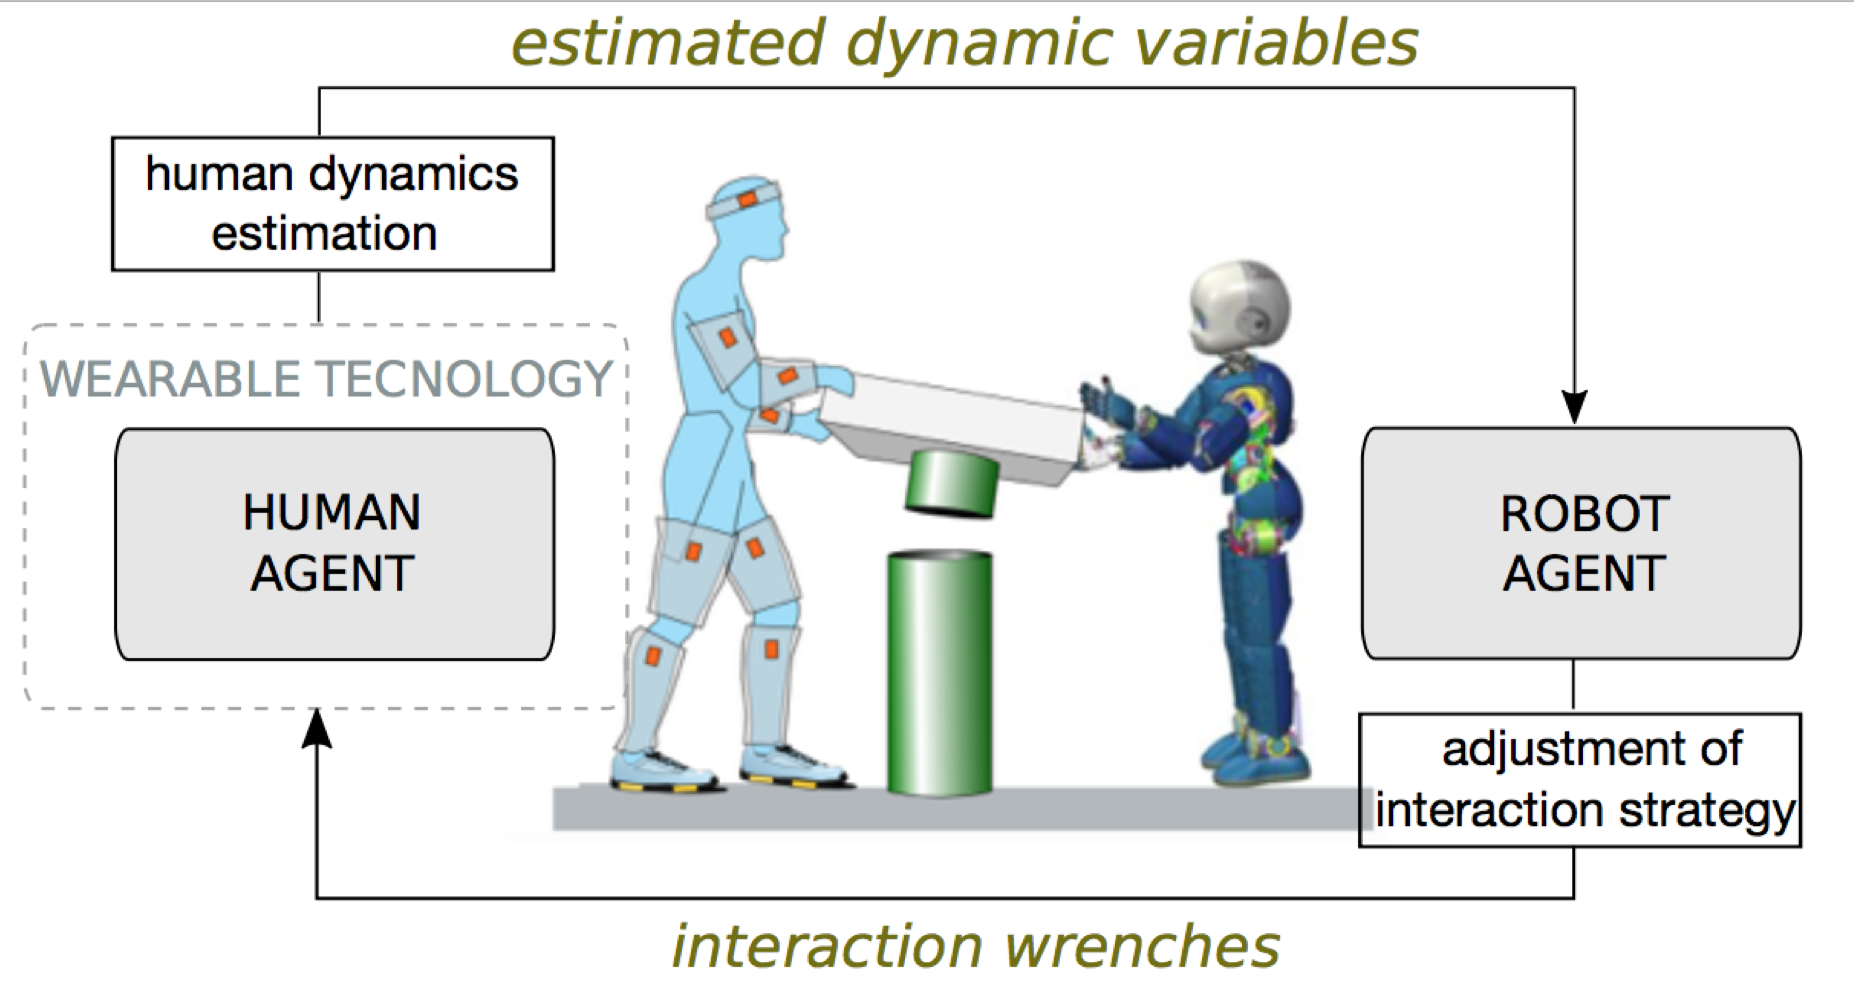
\includegraphics[width=1\columnwidth]{figs/schemeFramework}
  \caption{An example of pHRI scenario: the human agent is provided with a wearable 
  technology and an estimation algorithm allows to retrieve information about his dynamics. 
  By properly embedding estimations in the control loop of the robot, the 
  intentional collaboration may be enhanced.}
  \label{fig:figs_schemeFrameworkLoop}
\end{figure} 

%%%%%%%%%%%%%%%%%%%%%%%%%%%%%%%%%%%%%%%%%%%%%%%%%%%%%%%%%%%%%%%%%%%%%%%%%%%%%%%%%

\section{Problem Formulation}
\label{sec:problem}

	%%--------------------------------------------
%% Inverse Dynamics
%%--------------------------------------------
%Without contacts with the environment, 
The inverse dynamics of a robot with $m$ degrees of freedom can be generally described by 
%
\begin{align}
	\torques = \underbrace{\inertiaMatrix\ddq + \Hmatrix}_{\torques_\text{RBD}} + \epsilon\,(\q,\dq,\ddq) \,,
	\label{eq:tau_nocontact}
\end{align}
%
where $\q$, $\dq$ and $\ddq$ are  the joint positions, velocities and accelerations, respectively, 
%$\inertiaMatrix \in \R^{m \times m}$ is the inertia matrix and 
$\inertiaMatrix$ is the inertia matrix and 
%
\begin{align*}
	\Hmatrix = C(\q,\dq)\dq + g(\q) + F_v \dq + F_s \,\text{sgn}(\dq) %\in \R^{m \times m}
\end{align*}
%
is the matrix combining the contributions from Coriolis and centripetal, friction (viscous and static) and gravity forces.
The term $\epsilon(\q,\dq,\ddq)$ in \eq\eqref{eq:tau_nocontact} captures the errors of the model,
such as unmodeled dynamics (e.g., elasticities and Stribeck friction), inaccuracies in the dynamic parameters (e.g., masses, inertia), vibrations, couplings, and sensor noise. 
%
With a set $\mathcal{C}=\{c_1 \ldots c_n\}$ of contacts $c_i$ between the robot and the environment, \eq\eqref{eq:tau_nocontact} becomes
%
\begin{align}
	\torques = \underbrace{\inertiaMatrix\ddq + \Hmatrix}_{\torques_\text{RBD}} + \epsilon(\q,\dq,\ddq) + \sum_{c_i \in\mathcal{C}} {\jacobian\T_{c_i}(\q)}\, \extForces_i \, ,
	\label{eq:tau_contact}
\end{align}
%
where the last term accounts for the additive effect of the external wrenches (forces and moments) $\extForces_i$ applied at contact location $c_i$, and $\jacobian_{c_i}(\q)$  is the contact Jacobian\footnote{The contact location $c_i$ is not necessarily fixed as the contacts may occur on the whole robotic structure and not exclusively at the end-effectors. 
In such a case, the contact location, if not known a priori, must be estimated, typically through distributed tactile sensors.
To compute the contact Jacobian, we need the position of the contact point with respect to the reference frame of the link~\cite{Fumagalli2012}. Such a knowledge requires a kinematic calibration of the skin as explained in~\cite{DelPrete2011}.}.
%\todo[inline]{What exactly is a contact location? What coordinate
%  system? Explain these things}
%



\subsection{Classical model-based approaches for computing the robot dynamics}

Classical approaches for computing $\torques$ or $\torques_\text{RBD}$ rely on the dynamics model with known or identified kinematics and dynamics parameters~\cite{Ivaldi2014}. 
The torques $\torques_\text{RBD} = \inertiaMatrix\ddq + \Hmatrix$ can be computed analytically through the rigid body dynamics model of the robot, a standard parametric description of the robot~\cite{Featherstone2008}. 
The term $\epsilon(\q,\dq,\ddq)$ is often neglected, or implicitly taken into account by considering a perturbation in the dynamics parameters of $\torques_\text{RBD}$, which need to be identified accurately.




% \todo[inline]{ Fix this.
% 	The inverse dynamics does not have discontinuities. 
% 	However, the measurement noise is not homogeneous in the system, as measurement during contacts is much noisier than for free movements.
% 	Hence, the use of heteroscedastic models is well suited to the task and might provide huge benefits compared to standard homoscedastic models.}


%==> now we start with classical methods and robot identification.. etc etc
%The accuracy of the robot dynamics model therefore depends on the accuracy of its dynamics parameters.

Although parameter identification for industrial robots is relatively easy with exciting trajectories~\cite{Pedrocchi2014}, the procedure for floating-base robots, such as humanoids, is not straightforward because of two main issues: 
1) The generation of sufficiently large accelerations for the identification while maintaining the robot balance and the control of contacts. 
This issue was well explained by Yamane~\cite{Yamane2011calibration}, who proposed a technique to identify the mass and the local COM of the links in a humanoid robot with fixed feet at the ground and slow joint trajectories. 
2) The measurement of the external forces $\extForces_i$ exerted on the robot.
Note that it may not be straightforward to measure the external forces~$\extForces_i$ as it is not possible to cover the robot body with 6-axis force/torque sensors to measure the force exerted on every possible contact location $c_i$. 
Usually, such sensors are big, heavy and expensive.
Thus, they are carefully placed where the external forces are critical for the main tasks, for example at the end-effectors for manipulation and at the feet for balancing.
In such a case, it is possible to identify the dynamics parameters while balancing and walking without additional contacts~\cite{Ogawa2014}.
When force/torque sensors are placed proximally, such as in the \robot{} arms~\cite{Fumagalli2012}, some of the dynamics parameters can be identified, but in absence of contacts~\cite{traversaro2013inertial}.

When multiple contacts are exerted on the robot structure at locations other than the classical end-effectors, it is still possible to compute a precise inverse dynamics model, but this requires both pervasive joint torque sensing, such as in \textit{Toro}~\cite{Ogawa2014}, and additional force/torque and tactile sensing, such as in \robot{}~\cite{Ivaldi2011}.
Moreover, it requires the precise knowledge of the contact locations detected by the tactile sensors, which necessitates a spatial calibration of the skin~\cite{DelPrete2011}. 
This procedure is prone to errors, and it has been shown that small errors in the kinematics calibration of the taxels (i.e., the tactile units) can induce non-negligible errors in the estimation of the contact forces~\cite{DelPrete2012}.

Generally, these model-based approaches have three main limitations: 1) It is hard to add details about couplings, elasticity, friction and other nonlinear dynamics, which are required for high accuracy; 2) The performance of the data-driven identification strongly depends on the experimental setting (with/without contacts) and the exciting trajectories~\cite{Pedrocchi2014}; 3) They make strong assumptions to handle contacts.

%An alternative and appealing approach is to learn the dynamics model through machine learning techniques~\cite{Nguyen-Tuong2008,Vijayakumar2000}. 
%The main advantage of this approach has been clearly stated in \cite{Nguyen-Tuong2011}, where the authors showed that a learned dynamics could improve the performance of inverse dynamic control.

\subsection{Learning the inverse dynamics}

    %
    \begin{figure}[t]
        \centering
        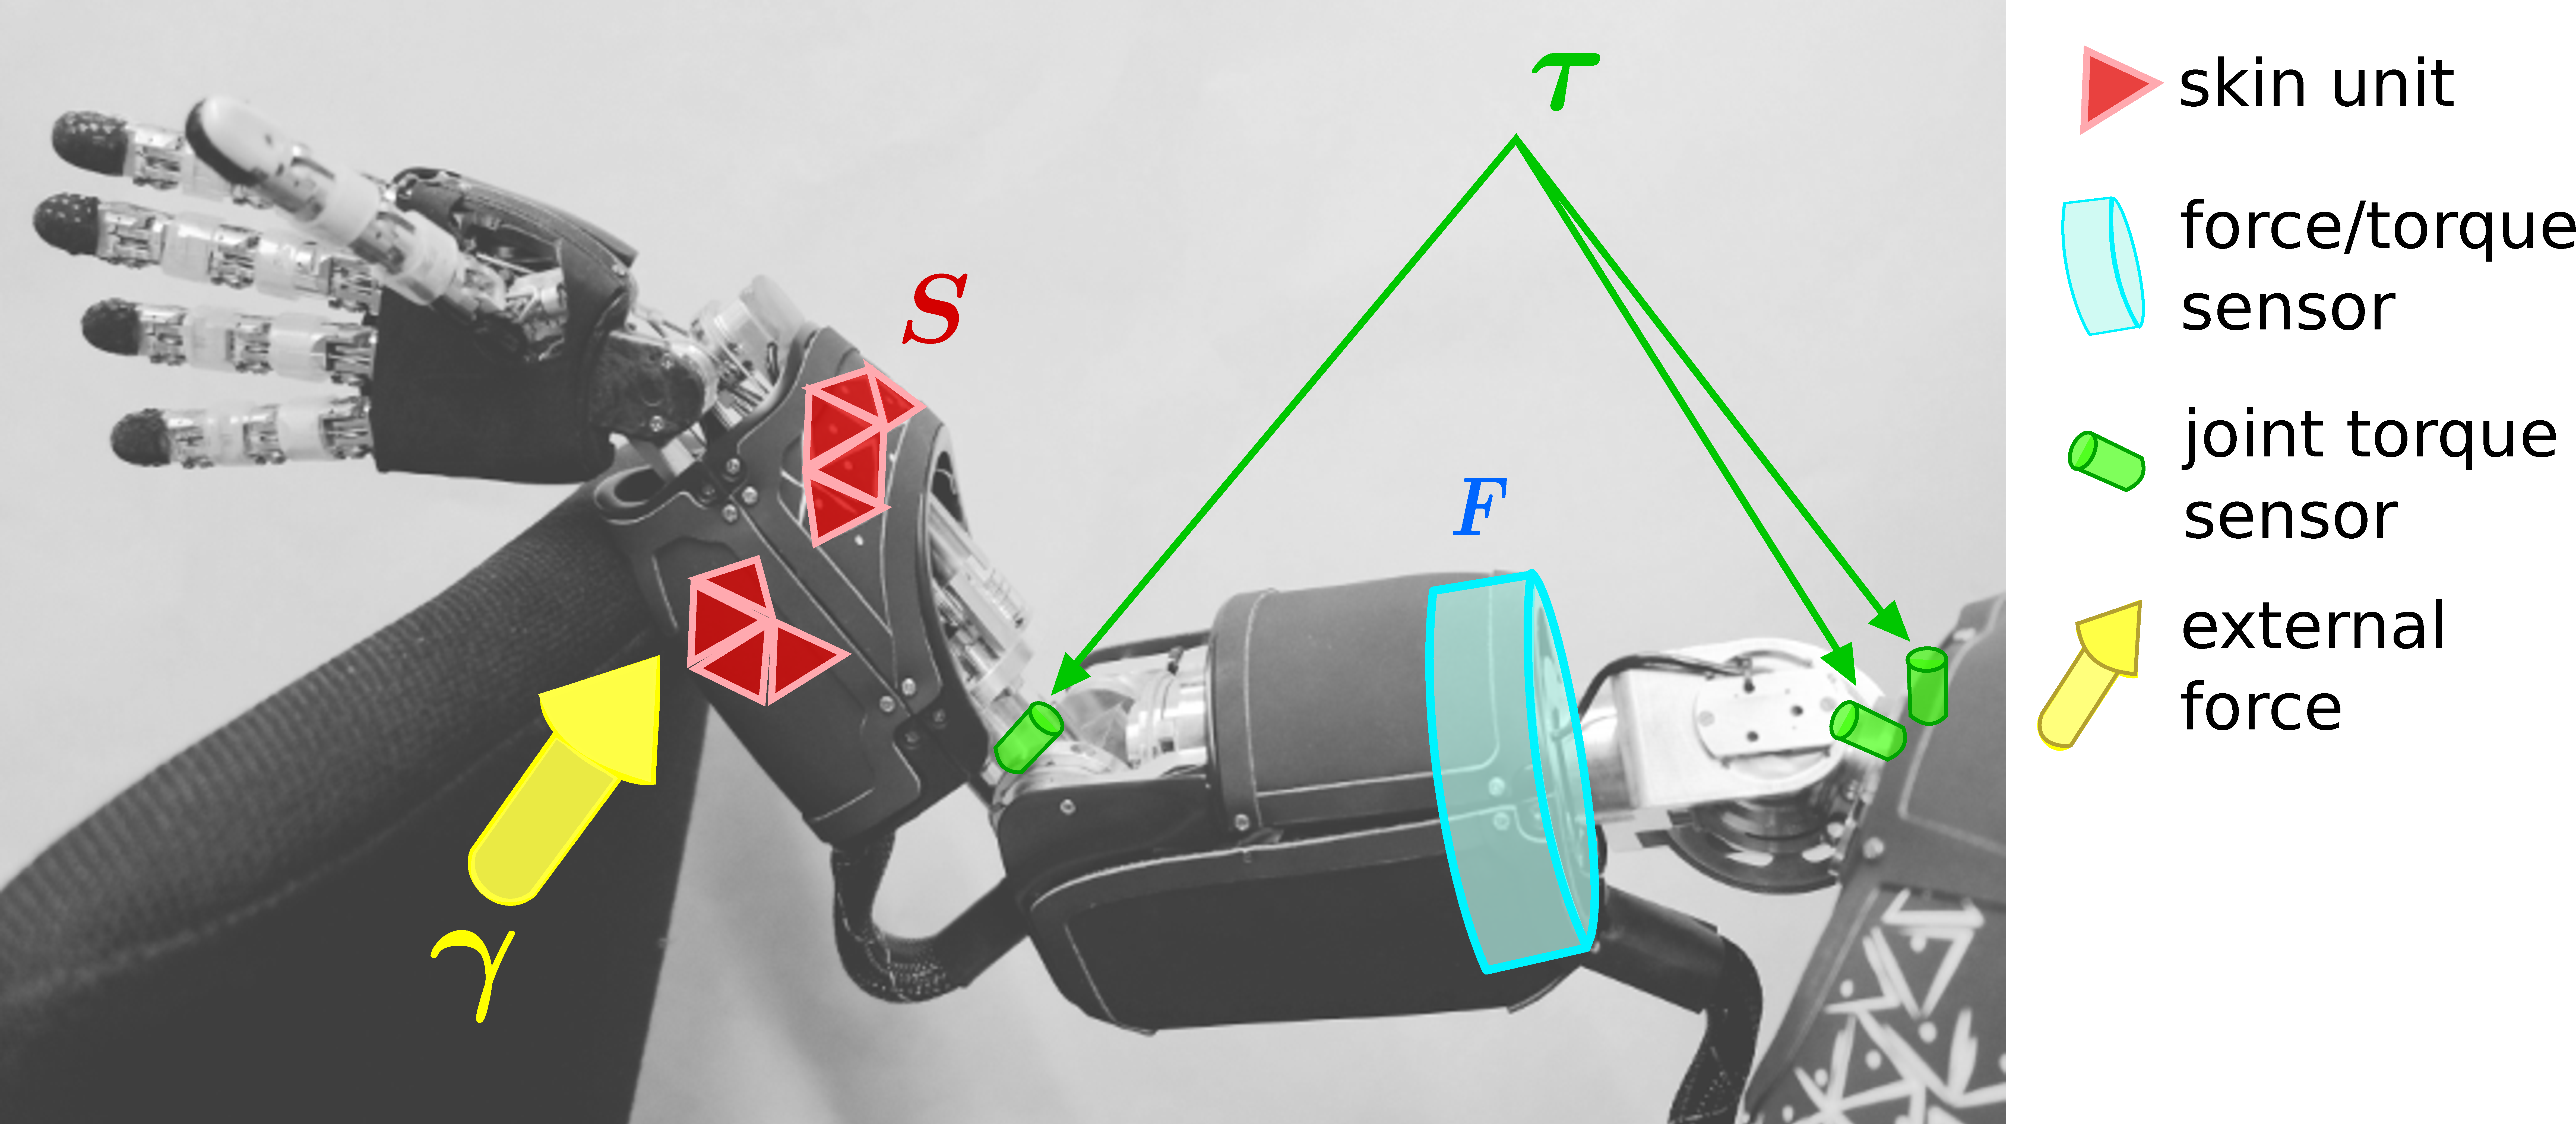
\includegraphics[width=.6\columnwidth]{robertoICRA/fig/concept_gray_new}		
        \caption{Illustration of the force/torque and tactile sensors during a contact of the robot arm with the environment.}
        \label{fig:concept}
        \figspace
    \end{figure}
    %
An alternative and appealing approach to analytic dynamics computation is to use machine learning methods to learn the dynamics model of a robot~\cite{Nguyen-Tuong2008,Vijayakumar2000,Deisenroth2012}. 
Without the need for compensating for inaccurate dynamics parameters and accumulated errors, a learned dynamics model can improve the tracking and control performances of a robot, as shown in~\cite{Nguyen-Tuong2011} for an industrial manipulator.
The clear advantage of learning the inverse dynamics is that we can overcome the limitations of the aforementioned approaches: difficulty in modeling complex nonlinear dynamics, impossibility to generate suitable exciting trajectories, restrictive assumptions regarding contacts and sensors, prior accurate kinematics calibration of the tactile sensors.
%\todo[inline]{Tricky statement. It depends on your model.}
%\todo[inline]{Unclear how learning overcomes these limitations}
%Several machine learning techniques have been applied to the problem of learning inverse dynamics, for example GP~\cite{???}, LGP~\cite{Nguyen-Tuong2008} and LWPR~\cite{Vijayakumar2000}.
%The better performance comes from the fact that we can easily learn unmodelled dynamics and the accumulated errors due to the inaccurate dynamics parameters. 
%For example, in \cite{Nguyen-Tuong2011} a learned dynamics could improve tracking performances in computed torque control for an industrial manipulator.
Despite the success of learned dynamics models in robotics, to the best of our knowledge there are no examples in the literature where dynamic contacts are also learned. 
%Prior works on learning or improving the inverse dynamics model lack a fundamental aspect: the inclusion of multiple contact dynamics in the model.
The inclusion of dynamic contact models in the dynamics highlights two main problems:
%There are two main problems.
First, switching from a no-contact model to a contact-model requires to observe the system state and to model a discontinuous function~\cite{Toussaint2005}. 
Second, switching between different contacts $c_i \in\mathcal{C}$ must be properly handled. %and to combine multiple ones simultaneously: that is dealing with a multitude of  $c_i \in\mathcal{C}$.\todo{unclear}

%
Here, we provide a first formulation to this problem, and we show that it is possible to learn the inverse dynamics model of the arm of the \robot{} robot by means of proximal force/torque measurements~$\ftsForces$ and distributed tactile sensors~$\skinInput$ (without requiring a spatially calibrated model of the skin~\cite{DelPrete2011}). 
%such that
%
%\begin{align}
%	\torques = \torques_\text{IDM}(\q,\dq,\ddq,\skinInput,\ftsForces) \,.
%\end{align}
%
%
% The benefit of such a model are many. 
% It only introduces an additional sensor measurement $\skinInput$, which provides the information about the contact location and a measure of the applied force on the taxel. 
% Tactile sensors are cheaper and lighter than force/torque sensors: with such a model, it can be possible to apply torque control to robotic manipulators in presence of dynamics contacts in locations other than the end-effector, which makes it possible to control physical interaction with an evolving environment or humans.
%This solution enables a fast and accurate prediction of joint torques in situations when the robot is in contact with none, one or even multiple simultaneous contacts, detected by a tactile skin.
%The estimation does not rely on dynamic parameters or parametric models, but is based on a data driven non-parametric model: Tactile sensors provide information about the contact locations (without requiring a spatially calibrated model of the skin~\cite{DelPrete2011}), while force/torque sensors provide information about the wrenches perceived by the robotic structure; joint torque sensors, here, provide the ground truth measurements.\footnote{If robots are not equipped with joint torque sensors, often it is possible to compute the joint torque through the motor current.}
%Our experiments are carried out on the humanoid robot iCub \cite{Natale2013}.

%We detail our proposed model and its learning procedure in the following section.
    
%%%%%%%%%%%%%%%%%%%%%%%%%%%%%%%%%%%%%%%%%%%%%%%%%%%%%%%%%%%%%%%%%%%%%%%%%%%%%%%%%

\section{Learning Inverse Dynamics with Contacts}
\label{sec:mgp}

	In this section, we present our proposed approach to learning inverse dynamics with contacts.
We first formalize the problem as learning a mixture-of-experts model.
Then we detail how we implement Gaussian processes as the corresponding experts.


\subsection{Learning contacts as a mixture-of-experts}
		%
	\begin{figure}[t]
		\centering
		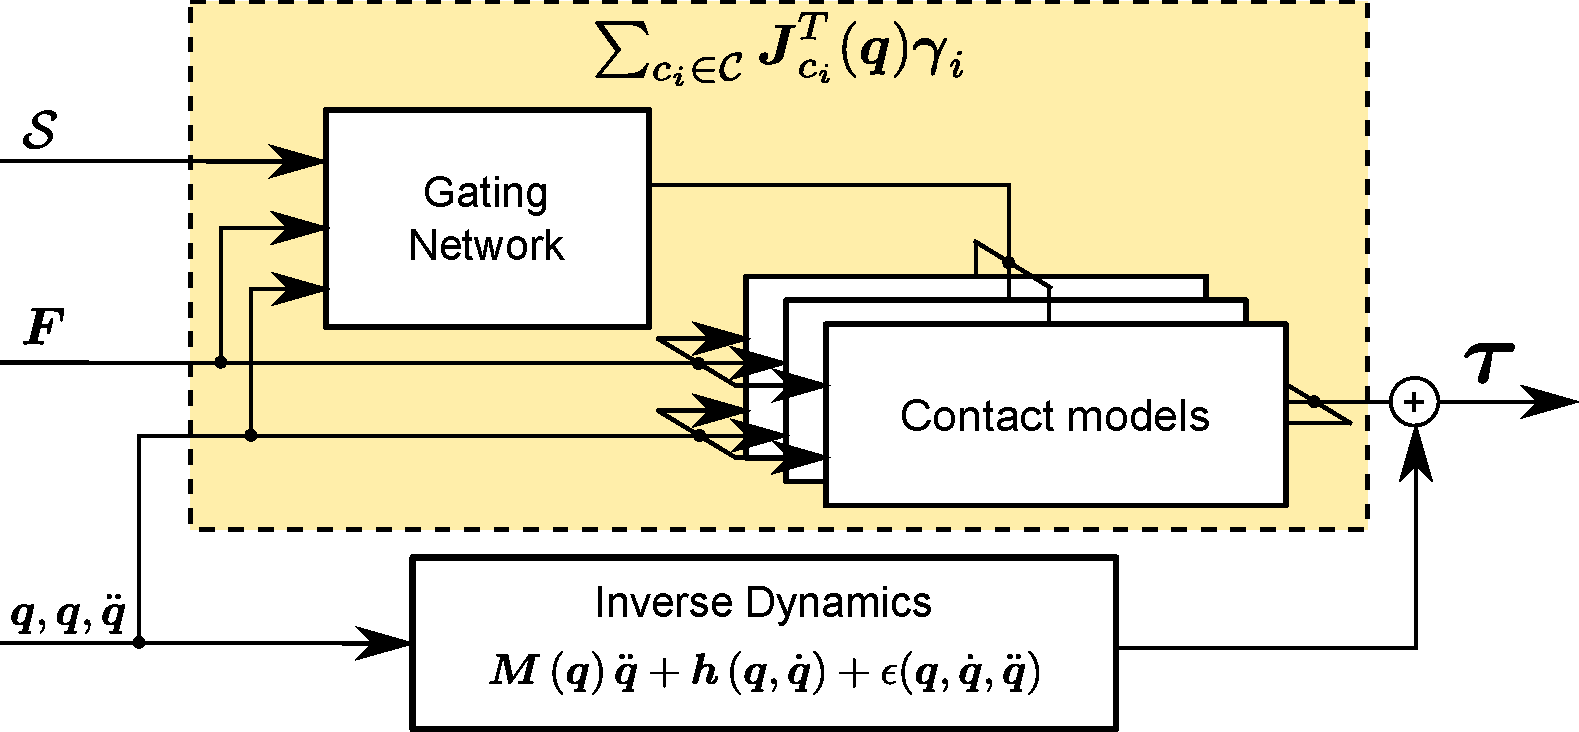
\includegraphics[width =.98\linewidth]{fig/diagram_2.pdf}
		\caption{Our approach extends existing inverse dynamics without contacts by learning many contact models, which serve as correction terms under different contact types. The decision of which contact model to activate is made by a gating network, which uses skin measurements~$\skinInput$, the force torque sensors~$\ftsForces$ and the current state $\q, \dq, \ddq$.}
		\label{fig:model}
        \figspace
	\end{figure}
	%
	When learning inverse dynamics with contacts \eq\eqref{eq:tau_contact}, we assume that the (contact-free) inverse dynamics from \eq\eqref{eq:tau_nocontact} can be computed precisely, either from an analytical model or from a learned model~\cite{Nguyen-Tuong2011}.
    %
    In our experiments, we employ a learned GP model as contact-free inverse dynamics.
    The reason for this choice are the unmodeled dynamics $\epsilon\,(\q,\dq,\ddq)$, which introduce substantial errors even without contacts.
	%
	As a result of the pre-existing contact-free inverse dynamics, only the model of the residual term of the external forces $\color{darkgreen}{\sum_{c_i \in\mathcal{C}} {\jacobian\T_{c_i}(\q)}\, \extForces_i}$ has to be separately learned.
    In this paper, we consider a robot that is provided with skin measurements~$\skinInput$ from the tactile sensors, force measurements~$\ftsForces$ from the force torque sensors (FTS) and the ground truth of the torques~$\torques$ from the joint torque sensors (JTS).
    An illustration of these relevant components is shown in \fig\ref{fig:concept}.
	Modeling the external forces $\color{darkgreen}{\sum_{c_i \in\mathcal{C}} {\jacobian\T_{c_i}(\q)}\, \extForces_i}$ can be formalized as the regression task
  	%
	\begin{align}
		\outputMatrix = \regressionNo([\q, \skinInput]) + \noise\,,
		\label{eq:regression}
	\end{align}
	%    
	where $\outputMatrix = \color{darkgreen}{\sum_{c_i \in\mathcal{C}} {\jacobian\T_{c_i}(\q)}\, \extForces_i}$ and  
    %$\inputMatrix = [\q, \skinInput,\ftsForces]$ are the inputs. 
	$\noise$ is an i.i.d. Gaussian measurement noise with mean~$0$ and variance~$\sigma_\noise^2$.
% 	Therefore, our regression problem is phrased as
%   	%
% 	\begin{align}
% 		\outputMatrix =\color{darkgreen}{\sum_{i \in\mathcal{C}} {\jacobian_i(\q)}\T \extForces_i} \color{black}{ = \regressionNo([\q, \skinInput,\ftsForces]) + \noise\,.}
% 		\label{eq:regression}
% 	\end{align}
% 	%    
	%
    Contacts with different parts of the body lead to different effects in the dynamics.
    Intuitively, it is necessary to consider the skin input~$\skinInput$ to identify the position of the contact.
	%It is necessary to consider the skin as an input~$\skinInput$ since contacts with different parts of the body lead to different effects in the dynamics.
	%Intuitively, $\skinInput$ is required to identify the position of the contact.
    Additionally, measurements of the force applied by the contacts are necessary to deal with a non-static environment.
    %\todo[inline]{Rephrase sentence above. It's unclear.}
    Theoretically, these measurements can be provided by the skin.
    However, the artificial skin used in our experiments does not provide a precise six-dimensional measure of the contact force.
	Therefore, in the implementation of our model we substitute the force measurement from the skin with the force/torque measurements~$\ftsForces$.
    The corresponding regression problem \eq\eqref{eq:regression} is complicated due to the high-dimensional space of the input $\inputMatrix \in \inputSpace$ (the skin measurements~$\skinInput$ alone account for hundreds of dimensions).
	Therefore, we rephrase this regression task as a problem of learning a mixture-of-experts model.
	With this model, we decompose \eq\eqref{eq:regression} as
	%
	\begin{align}
		\color{darkgreen}{\sum\nolimits_{c_i \in\mathcal{C}} {\jacobian\T_{c_i}(\q)}\, \extForces_i} \color{black}{ \,=\, \sum\nolimits_{j\in\mathcal{J}} f_j([\q, \ftsForces]) + \noise\,,}
		\label{eq:expertofmixtureregression}
	\end{align}
	%    
	where $\mathcal{J}$ is the set of active experts~$f_j$.
    %\todo[inline]{What is an active expert? Unclear.}
    %, which depends from $[\q, \skinInput]$.
	Note that the skin input~$\skinInput$ is no longer explicitly part of the inputs of the experts. %\todo{Why?}
    Therefore, each single expert~$f_j$ is now sufficiently low-dimensional to be modeled independently. At the same time the possibility of summing the contribution of each contact allows to account for complex%\todo{I don't like this word} 
    behaviors.
    As single expert~$f_j$ we use Gaussian processes for the mapping $[\q, \ftsForces] \mapsto {\jacobian\T_j(\q)} \extForces_j$.
    %Detailed information regarding the GP models and their training are given in the next subsection.
    A gating network is used to select the experts that are currently active and to add their contributions.    
    An illustration of our approach is shown in \fig\ref{fig:model}.
	%For mixture-of-experts models it is required to design a suitable gating network that activates the relevant experts.
    In this paper, we implement this gating network as a multi-class classifier $\mathcal{J} = g(\q, \skinInput,\ftsForces)$ that selects which contact is currently ongoing.
    %\todo[inline]{In a general setting, the gating network does not make hard decisions. Please make this clear. This would probably also change eq. (4) since you would need weights. }
	For simple tasks, this gating network can be designed using heuristics (e.g., using thresholds on the activation of the tactile sensors). 
    However, for more complex systems an adaptive, data-driven approach may be more suitable. 
    In the experimental section we evaluate the learning of such gating network.
    %\todo[inline]{Strange end of this section. Shall we delete it? It only adds confusion.}
	%This automatic design is increasingly helpful for high number of skin sensor ($>1000$), where the manual design became increasingly complex.

%\todo[inline]{How do you define the experts? And how many do you need? Not mentioned.}

%\todo[inline,color=yellow]{Make sure the section headings are consistently capitalized.}


\subsection{Gaussian processes as expert models}
%\todo[inline]{Introduce GPs only in the context of IDM: distribution over IDMs (instead of "function"), RBD as prior mean, define X and Y in this context immediately.}
	Gaussian Processes (GPs)~\cite{Rasmussen2006} are a state-of-the-art regression method.
	They have been used in robotics to learn dynamics models~\cite{Deisenroth2012} and for control~\cite{Deisenroth2014}.
    %
    In this paper, a GP is a distribution over inverse dynamics models 
	%
	%\begin{align}
		\mbox{$f \sim \GP \left( m_f,k_f \right) \,,$}
	%\end{align}
	%
	fully defined by a prior mean~$m_f$ and a covariance function~$k_f$.
	We choose as prior mean $m_f \equiv \torques_\text{RBD}$ and as covariance function~$k_f$ the squared exponential with automatic relevance determination and Gaussian noise
    %
	\begin{align*}
		{k(\vec x_p,\vec x_q)} &= \sigma_f^2\exp\left(\!-\!\tfrac{1}{2}(\vec x_p\! -\!\vec x_q)^T {\mat \Lambda\inv} (\vec x_p \!-\! \vec x_q)\right) \!+\! \sigma_\noise^2\delta_{pq}
		%\label{sec:GP:cov:SE}
	\end{align*}
	%
	where ${\mat \Lambda}=\diag([l^2_1,...,l^2_D])$ and $\delta_{pq}$ is the Kronecker delta (which is one if $p=q$ and zero otherwise). Here, $l_i$ are the length-scales, $\sigma^2_f$ is the variance of the latent function $f(\cdot)$ and $\sigma^2_\noise$ the noise variance. 
 %   The purpose of $\sigma_w^2\delta_{pq}$ is to model (and identify) the presence of the Gaussian noise~$\epsilon$.
 
    In our experiments, when learning contact models, the input is defined as $\parameters = [\q,\ftsForces]$, while the output (observations) $\vec y = \torques$ are the torques.
    Hence, given $n$ training inputs $\mat X=[\parameters_1,...,\parameters_n]$ and corresponding training targets $\mat y=[ y_1,..., y_n]$, we define the training data set $\dataset = \{\mat X,\mat y\}$. 
    % training
Training the GP corresponds to finding good hyperparameters $\vec \theta = [l_i, \sigma_f, \sigma_\noise]$, which is done by the standard procedure of maximizing the marginal likelihood~\cite{Rasmussen2006}.   
    
% predictive distribution    
    The GP yields the predictive distribution over torques for a new input $\vec x_* = [\vec q_*, \mat F_*]$
	%
	\begin{align}
		&\prob(\vec y|\dataset,\parameters_*,\vec \theta) = \gauss{\mu(\parameters_*)}{\sigma^2(\parameters_*)}\,, 
		\label{eq:one-step prediction distr}
	\end{align}
	%
	where the mean~$\mu(\parameters_*)$ and the variance~$\sigma^2(\parameters_*)$ are 
	%
	\begin{align}
		&\mu(\parameters_*) = \vec k^T_*\vec K^{-1} \mat y\,,\quad \sigma^2(\parameters_*) = k_{**}-\vec k^T_*\mat K^{-1}\vec k_*\,,
		\label{eq:one-step prediction mean and covariance}
		%\label{eq:one-step prediction cov}
	\end{align}
	%
	%% all the stuff from the equations
    respectively.	The entries of the matrix $\vec K$ are  $K_{ij}= k(\parameters_i,\parameters_j)$, and we define $k_{**}=k(\parameters,\parameters)$ and $\vec k_{*}=k(\vec X,\parameters)$.
    
    %\todo[inline]{It remains unclear how you use the GPs as experts in the MoE model. How do you determine the corresponding training data sets? What is the number of experts? And you also need to explain the gating network much better.} 
	
%%%%%%%%%%%%%%%%%%%%%%%%%%%%%%%%%%%%%%%%%%%%%%%%%%%%%%%%%%%%%%%%%%%%%%%%%%%%%%%%%

\section{Experimental Set-up and Evaluation}
\label{sec:results}

	% %
% \begin{figure}[t]
% 	\centering
% 	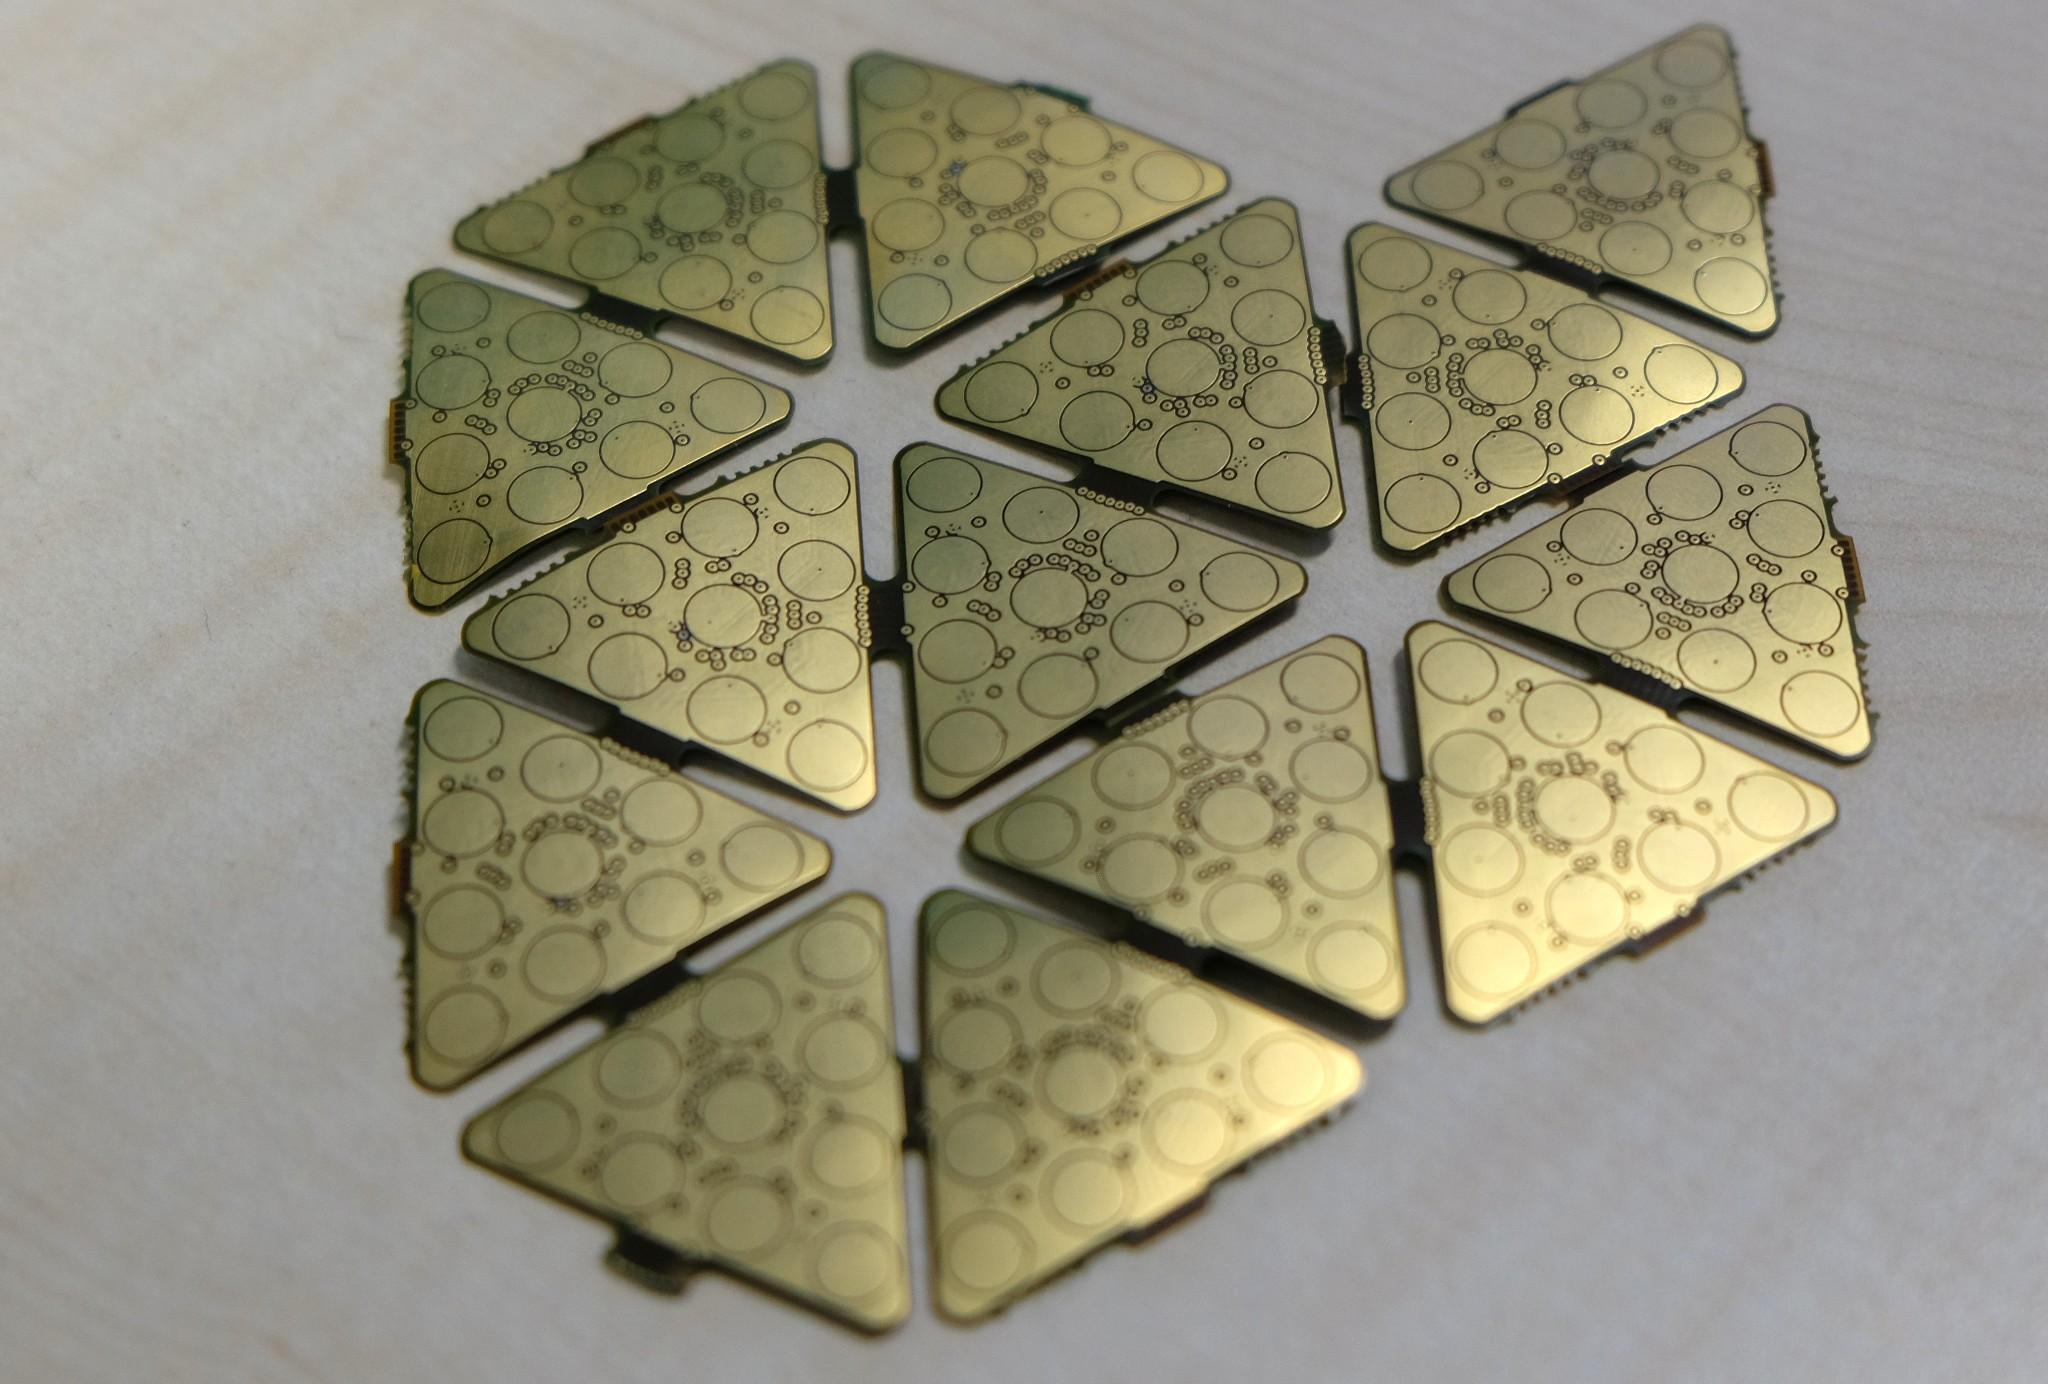
\includegraphics[width=.98\columnwidth]{fig/Skin1b}
% 	\caption{\robot{} Skin.}
% 	\label{fig:Fox_controller}
% \end{figure}
% %

%
% \begin{figure}[t]
% \resizebox{\hsize}{!}{
% 	\centering
% 	%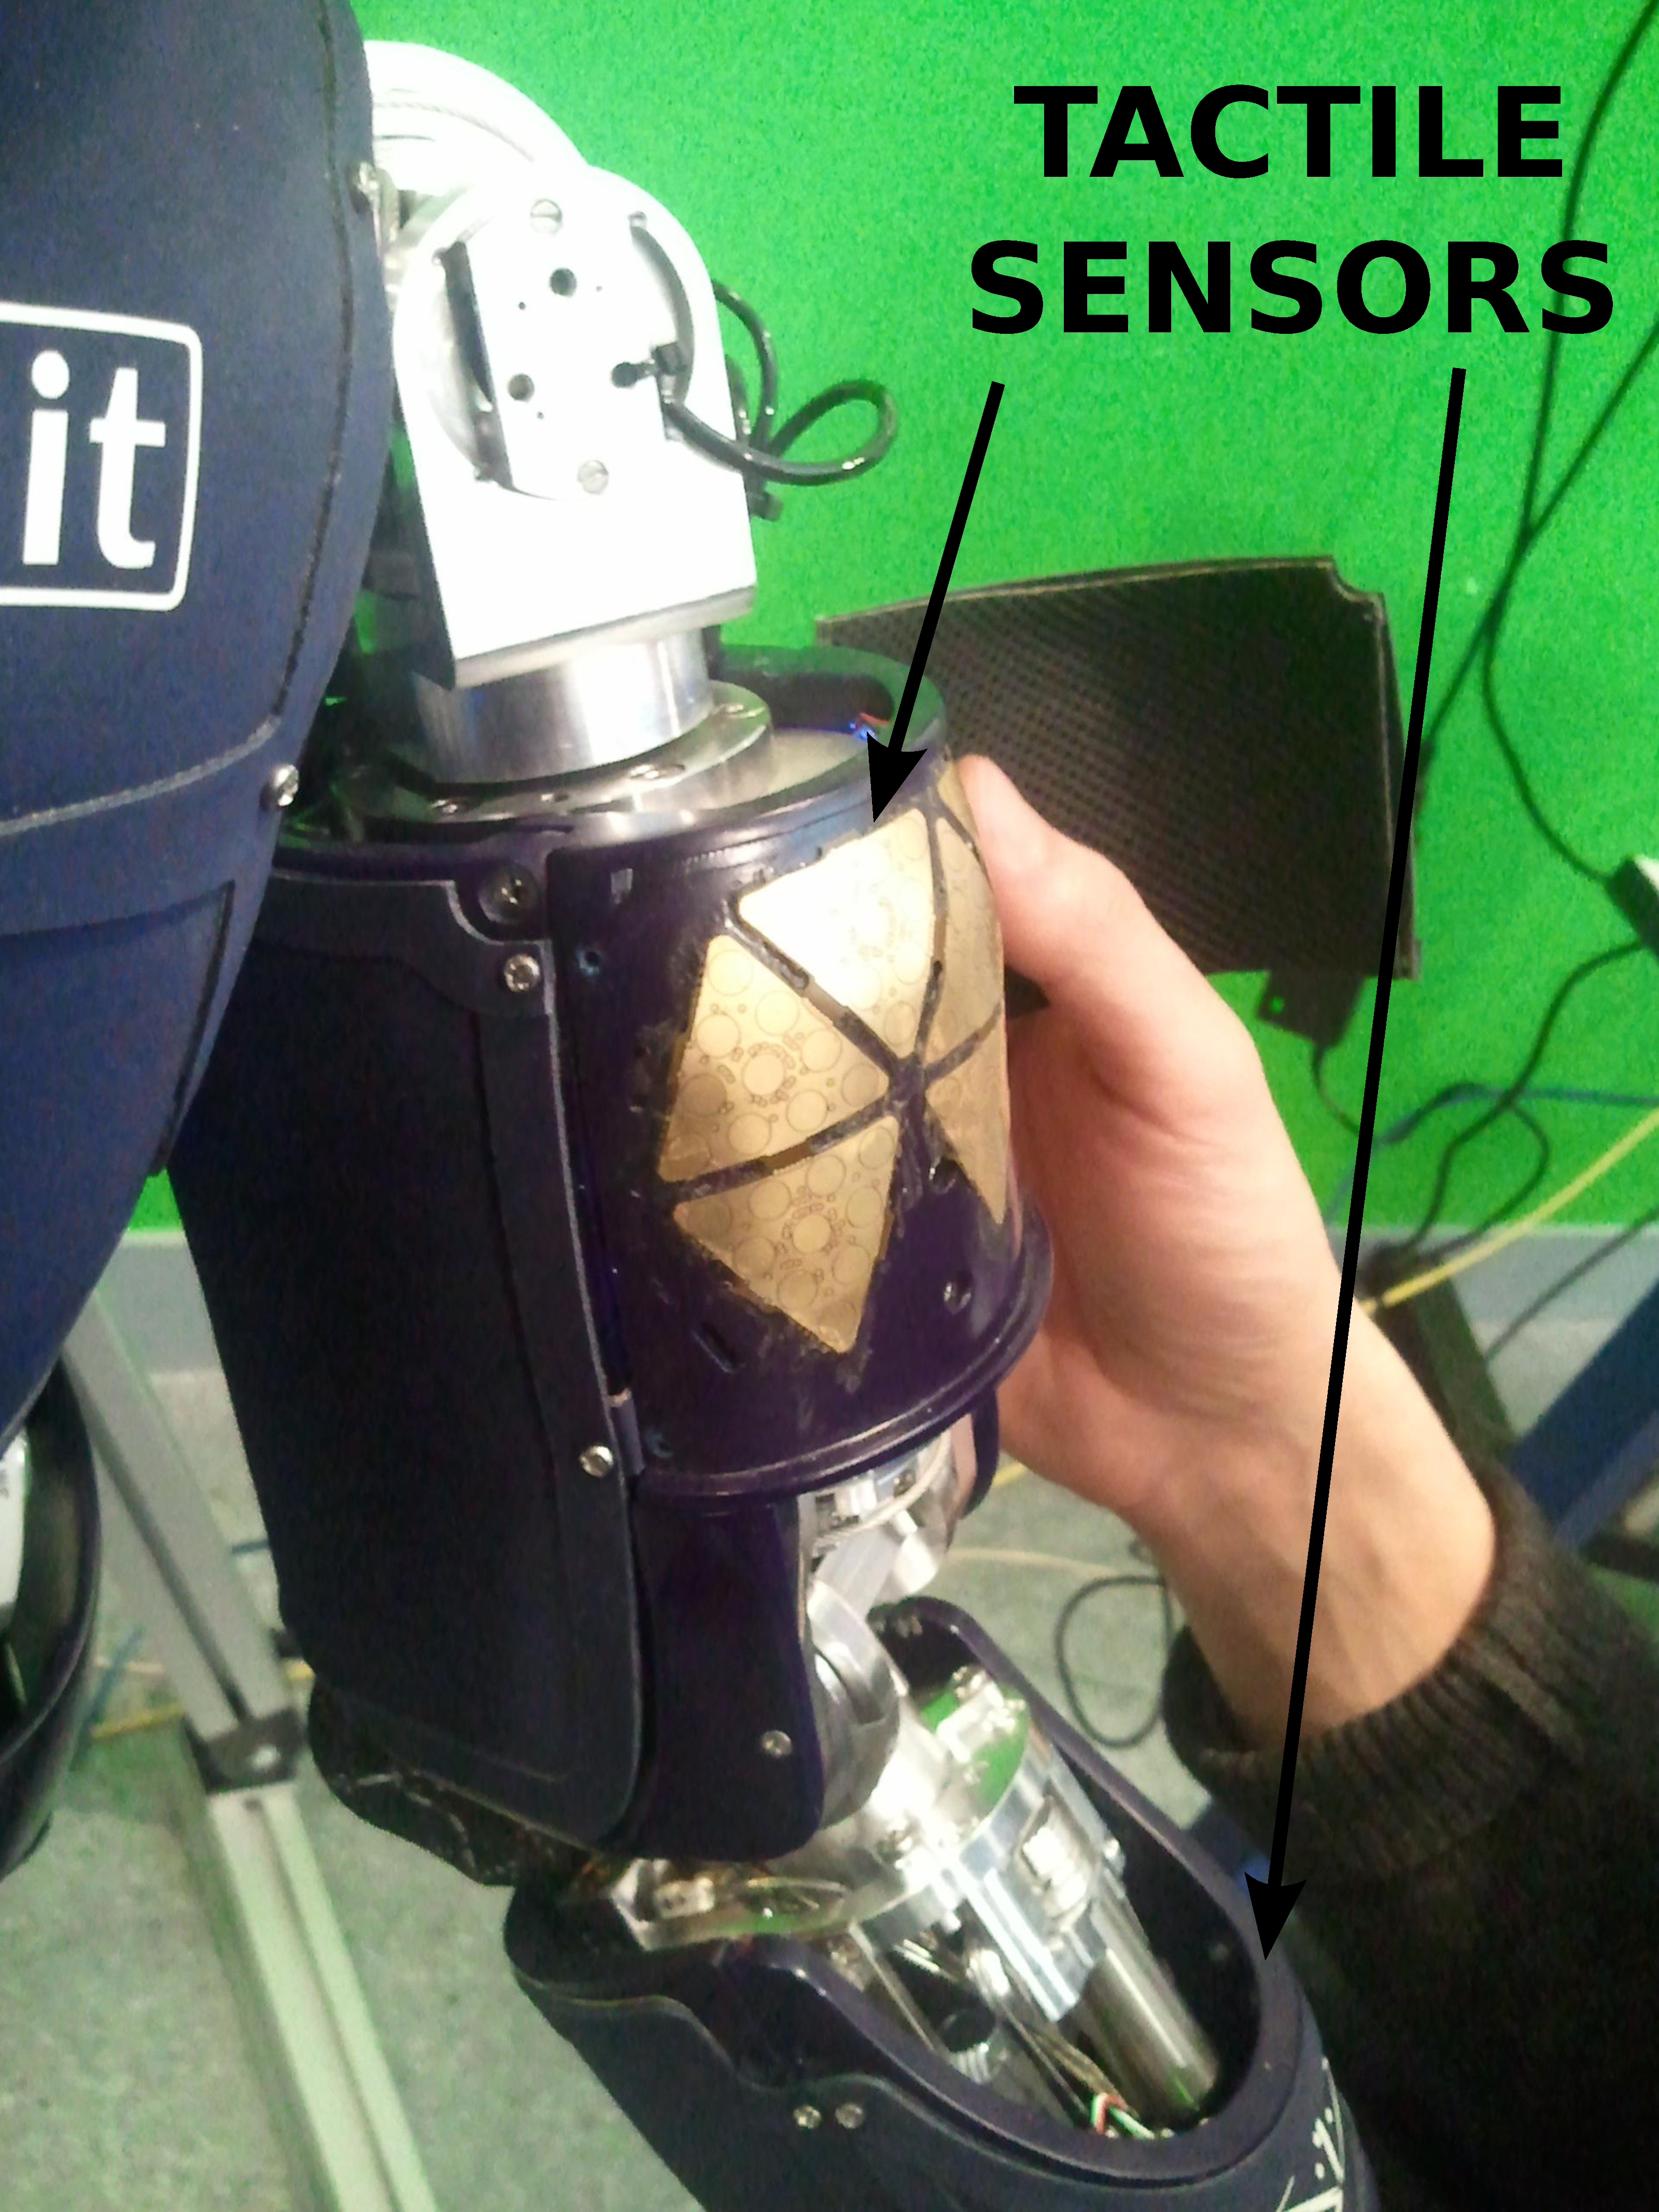
\includegraphics[height=4cm]{fig/icub_arm_skin_text}
% 	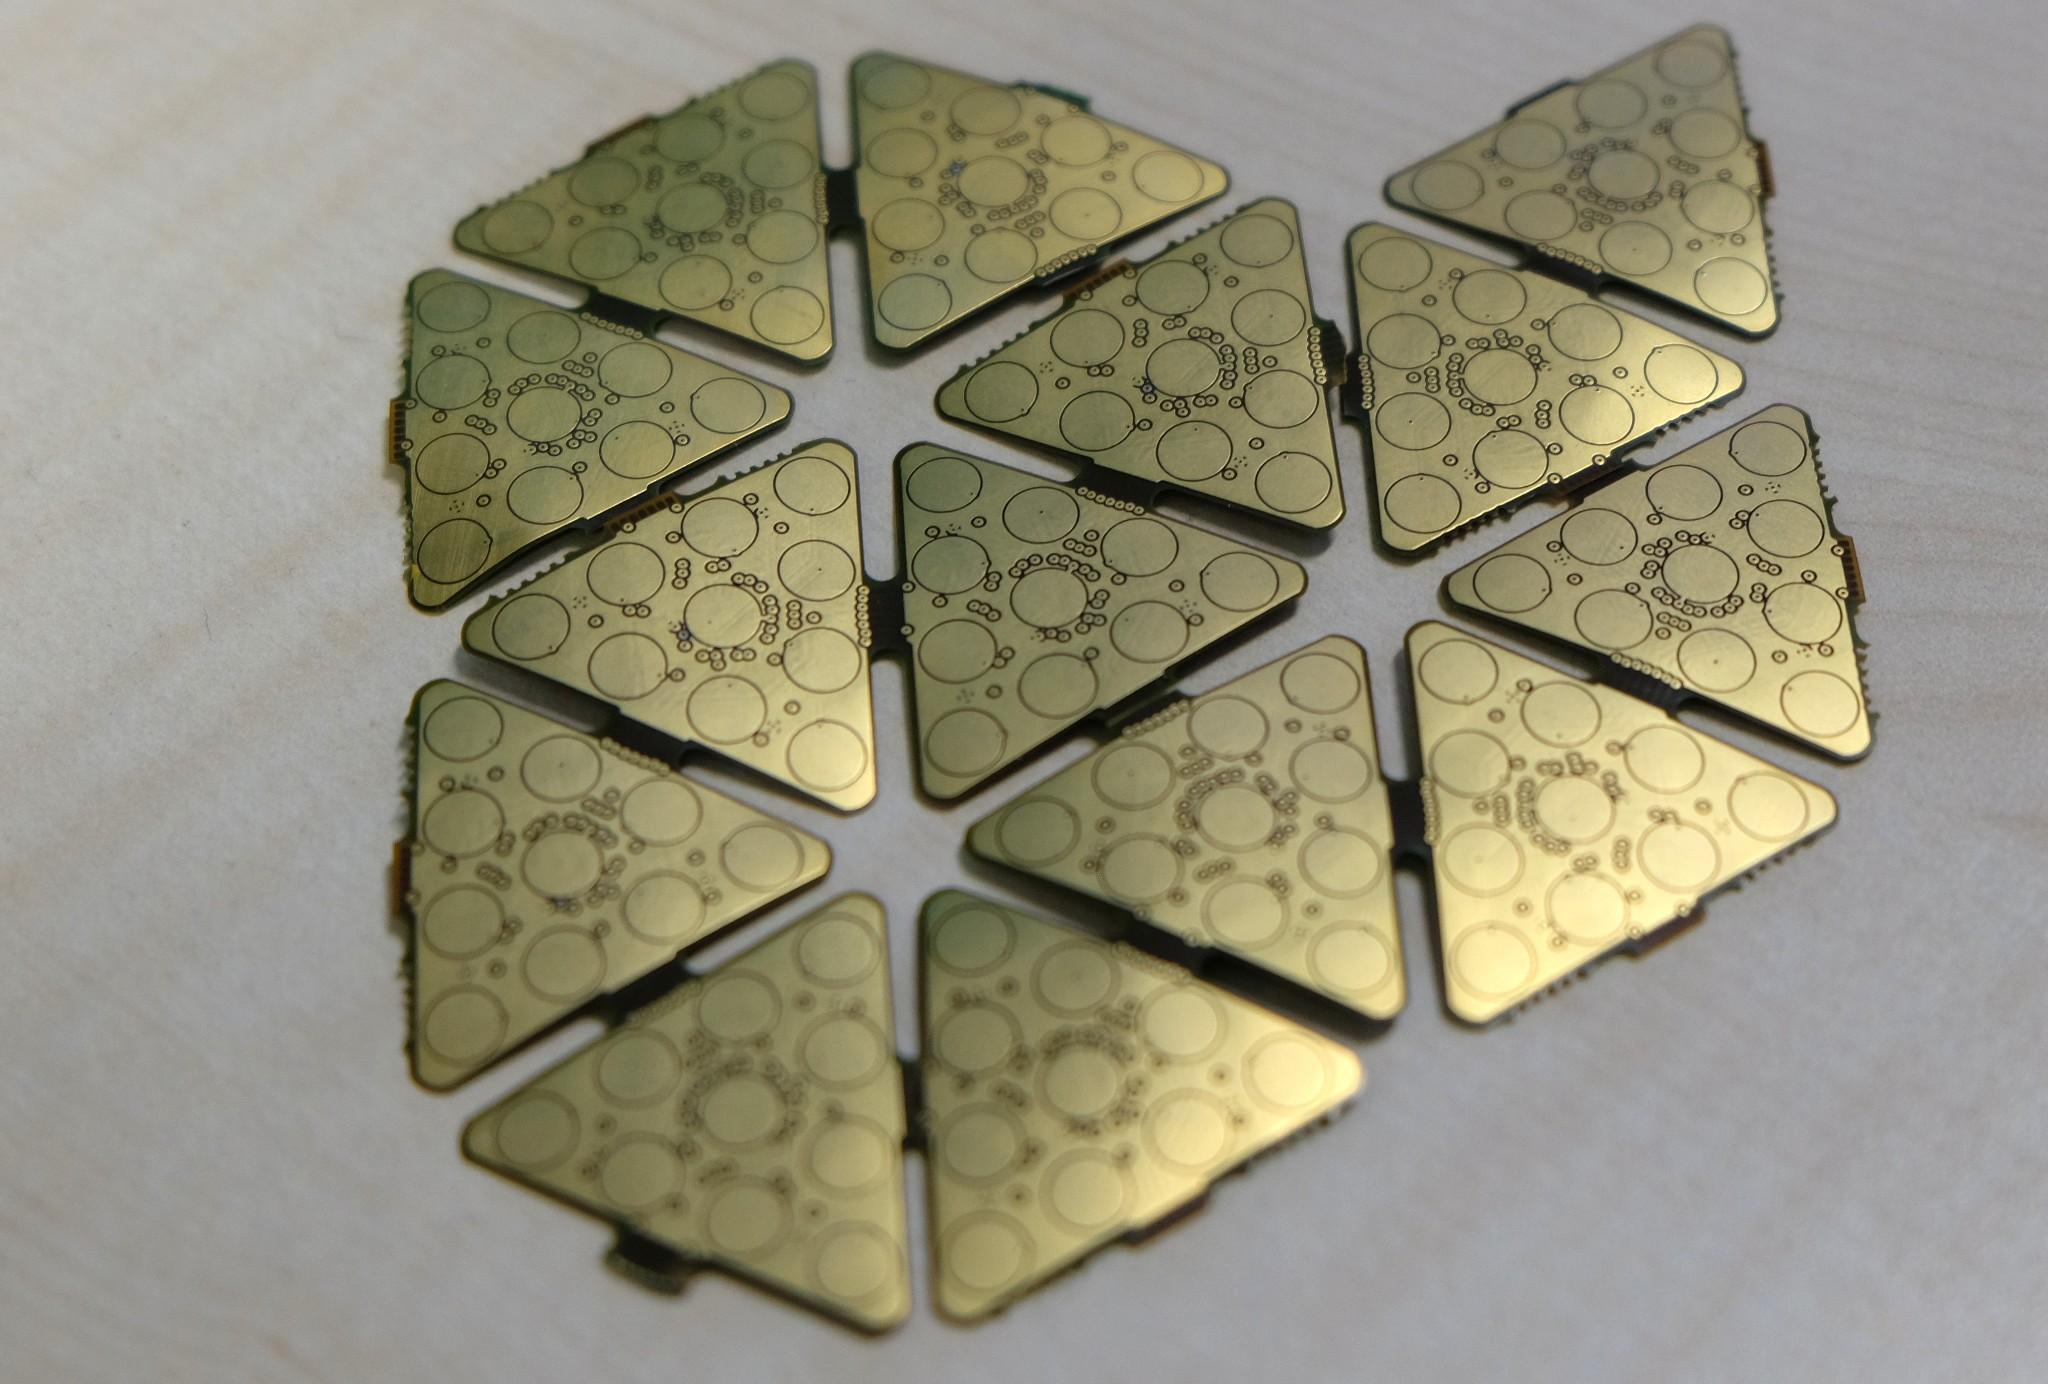
\includegraphics[height=4cm]{fig/Skin1b}
% 	\hfill
% 	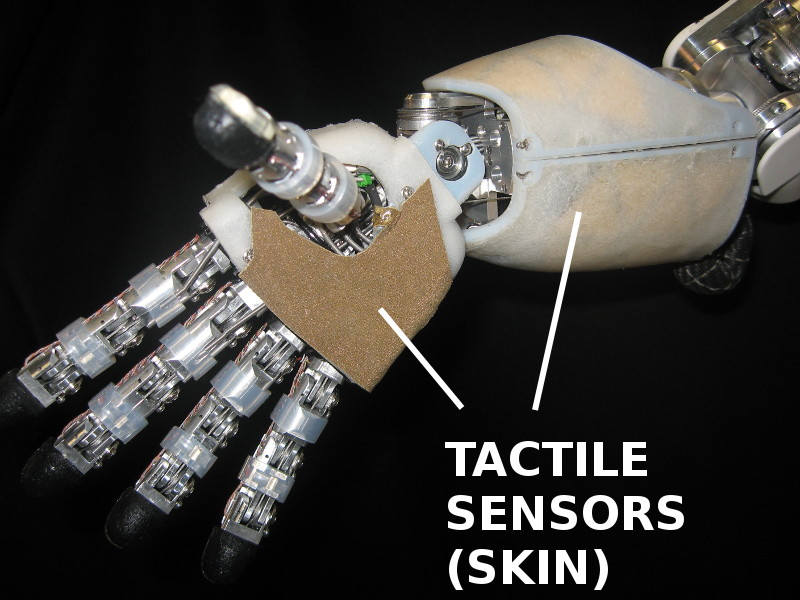
\includegraphics[height=4cm]{fig/icub_skin_arm_3}
% }
% 	\caption{The tactile elements (taxels) of the artificial skin covering the \robot{} arm. 
% 	Their measurements~$\skinInput$ are used to choose the appropriate expert.}
% 	\label{fig:icubskin}
% \end{figure}
%

%
	\begin{figure}[t]
		\centering
		\begin{subfigure}[t]{0.48\hsize}
			\centering
			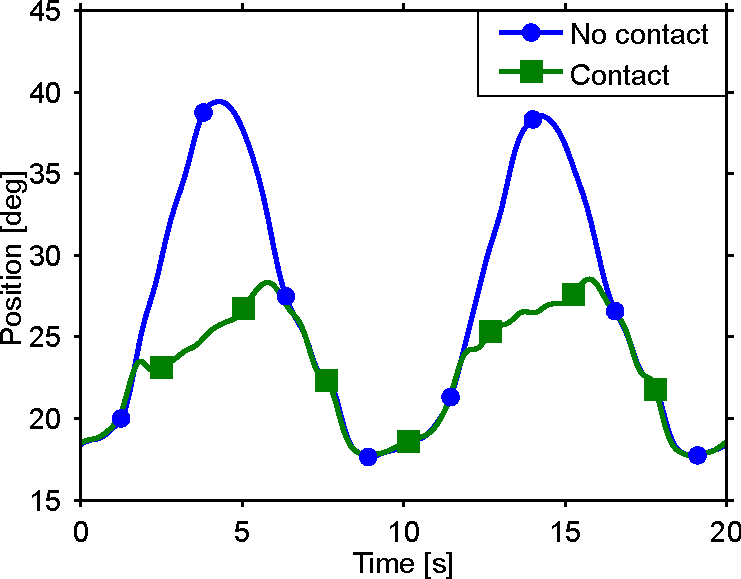
\includegraphics[height=3.2cm]{robertoICRA/fig/exp1_effectContactQ}%[width=.99\columnwidth]{fig/exp1_effectContactQ}
			\caption{Task space}
			\label{fig:exp1:effects_contact:a}
		\end{subfigure}
		\hfill
		\begin{subfigure}[t]{0.48\hsize}
			\centering
			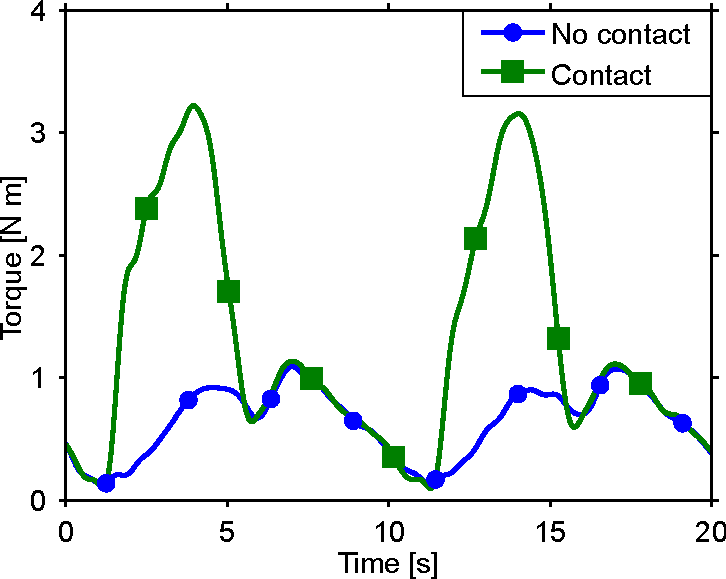
\includegraphics[height=3.2cm]{robertoICRA/fig/exp1_effectContactT}
			\caption{Torque}
			\label{fig:exp1:effects_contact:b}
		\end{subfigure}
		\caption{\textbf{\nameref{sec:results:exp1}:} Effects of a contact (green curve) compared to the free movement without obstacle (blue curve). 
		These effects are visible in the task space position~\subref{fig:exp1:effects_contact:a} and in the torque measured by the joint torque sensor~\subref{fig:exp1:effects_contact:b}.
		%\comment{Figures generated by \textit{Figures\_exp1}}
		}
		\label{fig:exp1:effects_contact}
        \figspace
	\end{figure}
	%


%% RESULTS
%we present the experimental results obtained.
 In this section, we describe the experimental setting and the humanoid robot~\robot{} used in the experiments.
% In the first experiment, we consider the case of learning a contact model for a fixed object. 
% In the second experiment, we demonstrate that a single contact model have generalization capabilities relatively to limited changes in the position of the contact.
% In the third experiment, we consider the case of multiple contacts. 
% We demonstrate that by combining models of single contacts it is possible to generalize to multiple contacts.
% In the fourth experiment, we consider a special case of multiple contacts: multiple simultaneous contacts.
% We show that our approach allows to sum the contributions from the single contacts to predict simultaneous multiple contacts.
% In the fifth experiment, we demonstrate that learning the gating network greatly reduce the design complexity, while achieve similar performances compared to a manual design.
%
We present four different experiments where we demonstrate that
1) Our approach can learn single contact models;
2) A single learned model (i.e., an expert) is robust to small changes in the position of the contact;
3) Our approach extends to multiple contacts by combining models of single contacts;
%4) our approach works even for multiple simultaneous contacts;\todo{check}
4) The gating network activating the experts can be learned to reduce the complexity of manually design it.

%===============================================================================


	

	

\subsection{Experimental set-up}

	%	
% 	\begin{wrapfigure}{r}{0.46\columnwidth}
% 	%\begin{figure}[t]
% 		\centering
%         \vspace{-10 pt}
% 		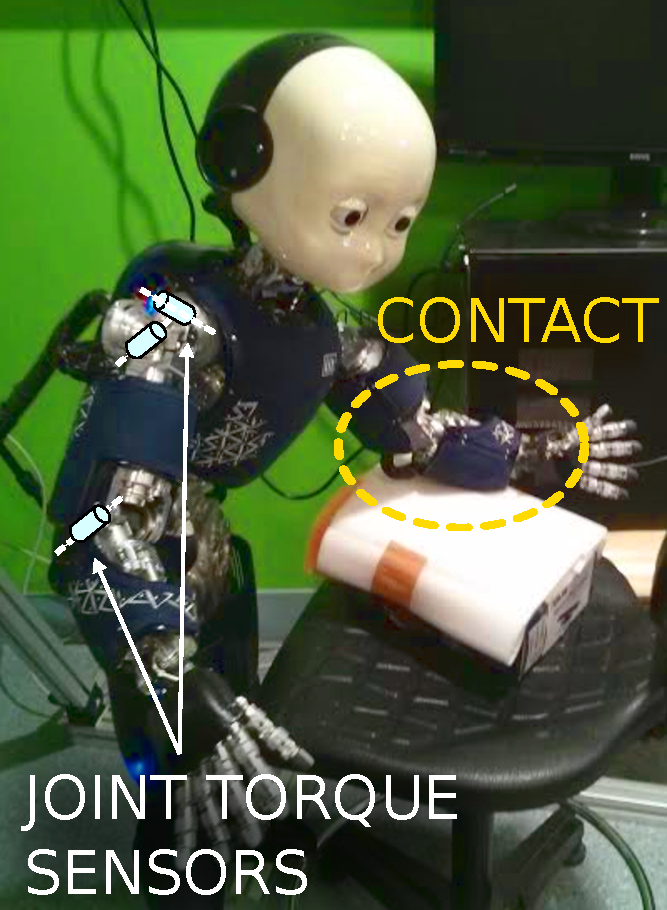
\includegraphics[width =\linewidth]{robertoICRA/fig/iCubParis02_contact_JTS}
% 		\caption{An experiment performed with iCub. The arm collides with the environment: the contact location is perceived by the skin in the forearm. On the left arm, the location of the three joint torque sensors is indicated.}
% 		\label{fig:icuparis_contact_jts}
% 	%\end{figure}
% 	\end{wrapfigure}
	%
	The experiments were conducted on the \robot{}~\cite{Natale2013}, a humanoid robot with 53 degrees of freedom, sized as a child (104 cm tall, 24 kg of weight).
	This robot is equipped with several sensors: an inertial sensor in the head, four 6-axis force/torque sensors placed proximally in the middle of legs and arms, and an artificial skin consisting of many distributed tactile elements (taxels) mounted on the robot covers~\cite{Cannata2008}. 
	The information from these three types of sensors is used to estimate the joint torques and the external contact forces by the \idyn{}  library~\cite{Ivaldi2011}. 
	In the following, $\torques_{\rm IDYN}$ denotes the joint torques estimated by the \idyn{} library, which we use as analytical model for comparison. 
	For more detail on its contact detection and taxels calibration we refer to~\cite{DelPrete2011,DelPrete2012}.
	%\comment{Still missing the explanation about why iDyn with multiple contacts is bad}

%	These sensors are used to detect the contacts, compute the external contact forces and estimate the joint torques~\cite{Fumagalli2012}. 
%	The tactile elements in the skin (see \fig\ref{fig:icubskin}) provide the information about the contact location; they also provide an indirect measure of the external force. 
%	The force/torque sensors, placed proximally in the middle of legs and arms, are used to estimate the robot dynamics (internal/external wrenches) and the joint torques.
%	This estimation is performed online by the library iDyn, which relies on the known dynamic model of the robot~\cite{Ivaldi2011}. 
%	\comment{Discuss the assumptions of the analytic model: ellipsoid thing}

 
	%Only one \robot{} was equipped with some joint torque sensors: precisely, iCubParis02 has three, placed in the first, second and fourth joint of the arm. 
	The \robot{} used in the experiments is equipped with three additional Joint Torque Sensors (JTSs), two in the shoulder and one in the elbow.
	The JTSs are calibrated by computing the offset and gain trough least-square regression with respect to the output of~\idyn{}.
	We consider these calibrated JTSs as ground truth measurements of the joint torques~$\jtsForces$.
	%\fixme{To calibrate the JTS, we compute the offset as the difference in absence of movement and the gain using Least-Square regression on the data.}
	%%The \robot ~\cite{Metta2008} is a humanoid robot with \fixme{N} degrees of freedom.
	%These skin sensors measure values correlated with the pressure applied to the skin itself.
	%
    	In our experiments, we used the \robot{} torso and arms (3 and 7 degrees of freedom, respectively) and the skin input~$\skinInput$ from the forearm, which consists of 270 sensor measurements.


%===============================================================================

%
	\begin{figure}[t]
		\centering
		\begin{subfigure}[t]{0.48\hsize}
			\centering
			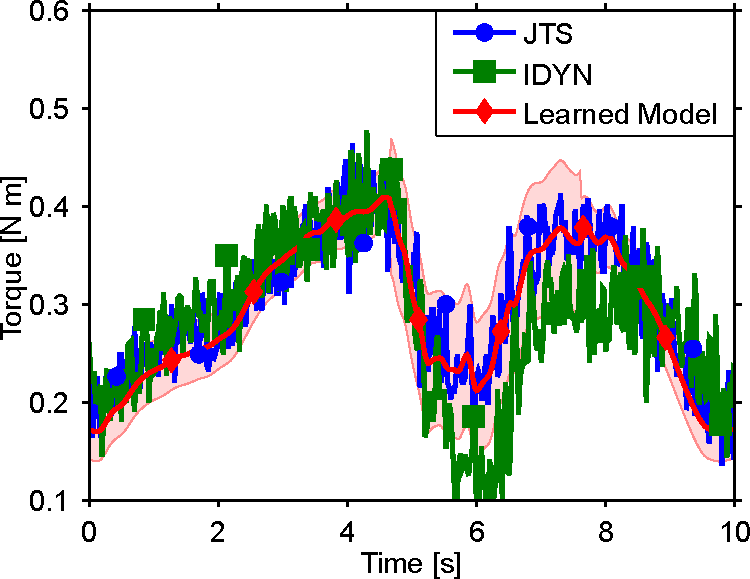
\includegraphics[width=.69\columnwidth]{robertoICRA/fig/exp1_model_notfilt}
			\caption{Real data.}
			\label{fig:exp1:model_contact:a}
		\end{subfigure}
		\hfill
		\begin{subfigure}[t]{0.48\hsize}
			\centering
			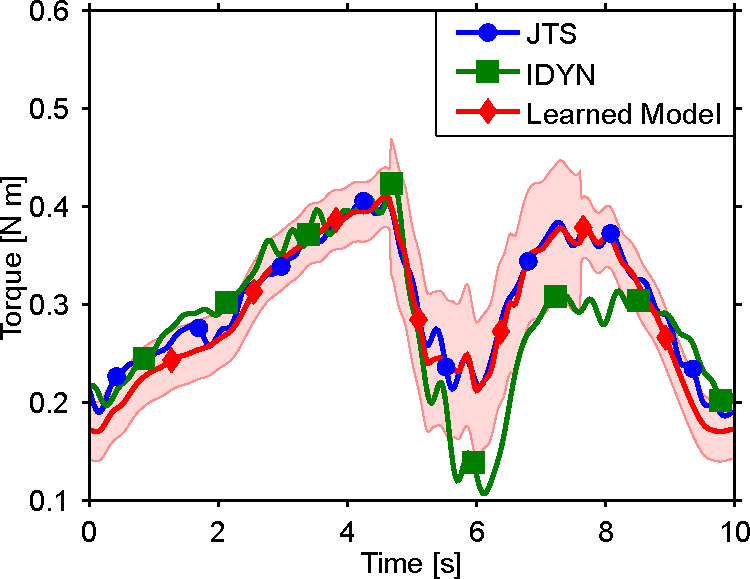
\includegraphics[width=.69\columnwidth]{robertoICRA/fig/exp1_model_filt}
			\caption{Filtered visualization.}
			\label{fig:exp1:model_contact:b}
		\end{subfigure}
		\caption{\textbf{\nameref{sec:results:exp1}}: Comparison of the torque measured at the elbow (with contact) by the JTS,  estimated by \idyn{} and our learned model (shown as $\text{mean}\pm 2\,\text{std}$). 
		Our learned model better predict the torque measured by JTS~\subref{fig:exp1:model_contact:a}.
		Additionally, due to the identification of the noise in the model, its prediction is smoother compared to both the noisy JTS measurements and the prediction from \idyn{}.
		For visualization purposes we also show the predictions when filtering JTS and \idyn{}~\subref{fig:exp1:model_contact:b}.
		%\comment{Figure generated by \textit{SomeFigures}}
		}
		\label{fig:exp1:model_contact}
        \figspace
	\end{figure}
	%
    	% 
	\begin{table}[t]
		\resizebox{\hsize}{!}{
		\centering
		\begin{tabular}{|l|l|c|c|c|}
			\hline 
			& Method	& Shoulder 1 [Nm] & Shoulder 2 [Nm] & Elbow [Nm] \\
% 			\cline{2-7}
			\hline 	
			\multirow{2}{*}{Full trajectory}  & \idyn{} & $0.09 \pm 1.1 \times 10^{-3}$ & $0.16 \pm 1.8 \times 10^{-3}$ & $0.05 \pm 7.4\times 10^{-4}$ \\ 
			& Our model 		& $\mathbf{0.04  \pm 5.6 \times 10^{-4}}$ & $\mathbf{0.07  \pm 9.8\times 10^{-4}}$ & $\mathbf{0.02  \pm 3.1\times 10^{-4}}$ \\
			\hline
			\multirow{2}{*}{Contact only}  & \idyn{} 	& $0.07 \pm 3.1 \times 10^{-3}$ & $0.13 \pm 5.7 \times 10^{-3}$ & $0.08 \pm 3.0 \times 10^{-3}$\\ 
			& Our model 		& $\mathbf{0.03  \pm 1.5 \times 10^{-3}}$ & $0.12  \pm 5.9 \times 10^{-3}$ & $\mathbf{0.03  \pm 1.3 \times 10^{-3}}$ \\
			%\cline{2-7}
			\hline
		\end{tabular}
		}
		\caption{\textbf{\nameref{sec:results:exp1}:} Mean and standard deviation of the mean for the RMSE of the test set for ground truth, predictions with the \idyn{} and our learned model. 
		The learned model predicts the torque more accurately than~\idyn{} for both the full trajectory and  during the only contact phase.
		}
		\label{tab:exp1}
        \figspace
	\end{table}
	%

\subsection{Learning a single contact}
\label{sec:results:exp1}


	In this experiment, we consider the \robot{} making contact with a single obstacle.
	%
	%% objectives of the experiment
	The evaluation is performed on a simple tracking task with the \robot{}'s end-effector moving along a circular trajectory.
	We repeat the task twice: first without any contact and then with a contact at a fixed position.
\fig\ref{fig:exp1:effects_contact} shows the effects of the contact in terms of position and torque during the tracking task. When the contact occurs the position error increases considerably. As a result, the torque is increased to compensate for the obstacle. 
	We collected 10 repetitions of the trajectory with the contact and used 8 of them to train the model.
    %We down-sampled the data to 40 Hz for a total of 939 data points, in order to reduce the computational time.
	The remaining trajectories are used as test set to evaluate the predictive performances of our learned model.
    For this experiment we consider a single expert (the gating network still decides whether to activate the expert).
    
    
    %We assess the quality of a learned contact model compared to the classical inverse dynamics model $\torques(\q,\dq,\ddq)$.
	We compare the baseline joint torque (measured by the JTS) to the joint torque estimated by the analytic model \idyn{} and  the joint torque $\torques_\text{IDM}$ predicted by our learned model.
	In \tab\ref{tab:exp1}, we report the root mean square error (RMSE) and the standard deviation of the mean of \idyn{} and our learned model for all the three joints.
	Additionally, we report both the error of the learned models (learned RBD plus learned contact model) during the full trajectory and exclusively \textit{during} the contact. 
	In five out of six cases, the learned model performs better than the analytic model. 
    In the sixth case (contact only, shoulder 2), the performance of the learned model is similar to the analytic model.
    However, increasing the amount of data used for training may further increase the performance of the learned model. 
    %\todo[inline]{Sounds funny: it's only similar because of small training data set size. Otherwise it should be worse? BTW: what is the training set size?}
	%We hypothesize that the performance of the learned model is due to the limited amount of data used for training.
	%In the following experiments, where more data was collected, the prediction accuracy for shoulder 2 improves in line with shoulder 1 and the elbow.
	%Failing to do so, would further decrease the performances of \idyn{}, due to the previously mentioned prediction error in the RBD.
	A visual representation of the predictions of the test set for the elbow joints is shown in~\fig\ref{fig:exp1:model_contact}.
	
    This experiment provides evidence that the classical rigid-body dynamics model $\torques_\text{RBD}(\q,\dq,\ddq)$ and the \idyn{} estimation (that also exploits proximal force/torque sensing) fail to accurately estimate the joint torques when the robot is in contact with the environment. 
	%Therefore, we need to include the contact information in such a model, i.e., $\torques_\text{IDM}(\q,\dq,\ddq,\skinInput,\ftsForces)$.
	Moreover, we show that the learned contact model, when combined with the RBD model, provides a better approximation of the joint torque.
	

% 	%
% 	\begin{figure}[t]
% 		\centering
% 		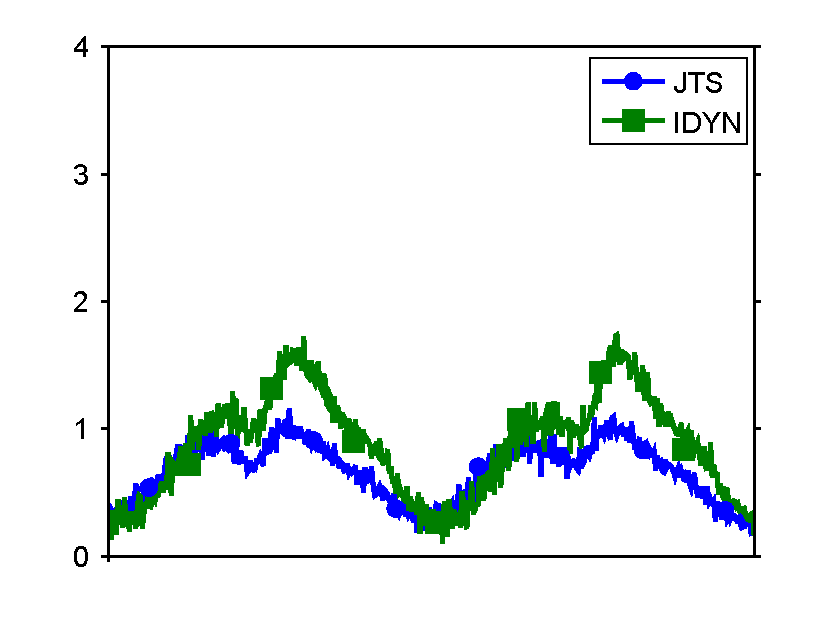
\includegraphics[width=.99\columnwidth]{robertoICRA/fig/exp1_contact}
% 		\caption{\textbf{\nameref{sec:results:exp1}}: the comparison, in absence of contact, of the torque measured by the JTS, the one estimated by iDyn using the FTS and the one generated by combining the RBD model with the learned model. \comment{Figure generated by \textit{SomeFigures}}}
% 		\label{fig:exp1:model_nocontact}
% 	\end{figure}
% 	%



%===============================================================================


\subsection{Robustness of the single contact model}
\label{sec:results:exp2}

% %
% 	%\begin{figure}[t]
% 		\begin{figure}[t]
% 		\begin{minipage}{.46\linewidth}
% 		\centering
% 		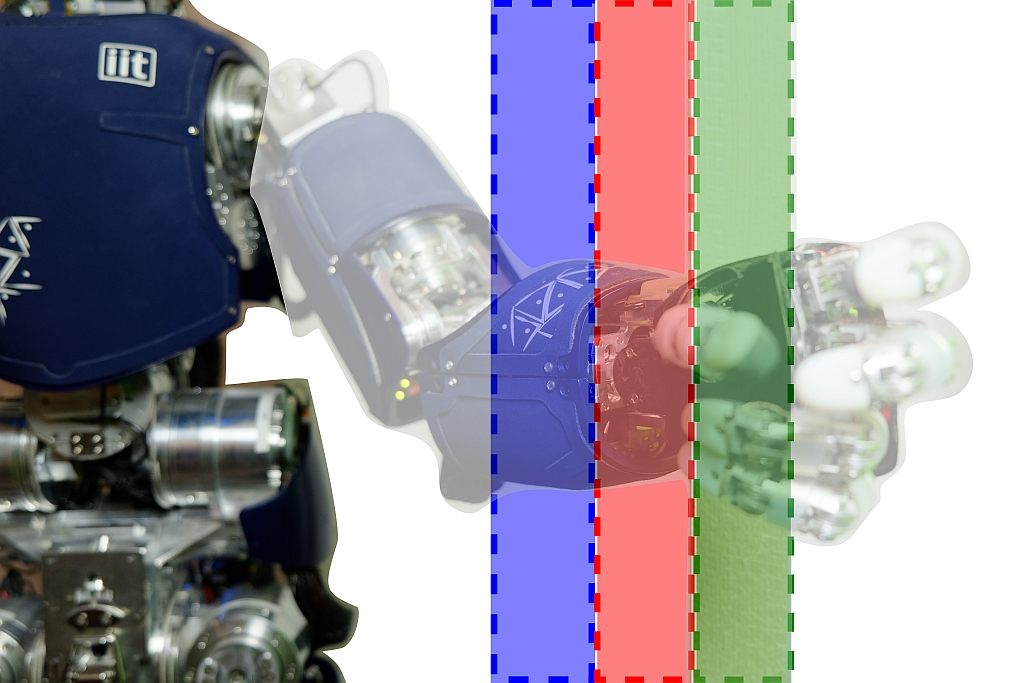
\includegraphics[width=.99\hsize]{robertoICRA/fig/Generalized_01}
% 		\caption{\textbf{\nameref{sec:results:exp2}}: The robot performs a movement with the left arm. The forearm collides with one of the three different obstacle: \textcolor{blue}{contact 1 (far)}, \textcolor{red}{contact 2 (medium)} or \textcolor{darkgreen}{contact 3 (close)}}
% 		\label{fig:exp2:robot}
% 	%\end{wrapfigure}
% 	%\end{figure}
% 	%
% 	\end{minipage}
% 	\hfill
% 	\begin{minipage}{.50\linewidth}
% 	 	%
%  	%\begin{figure}[t]
% 		\centering
% 		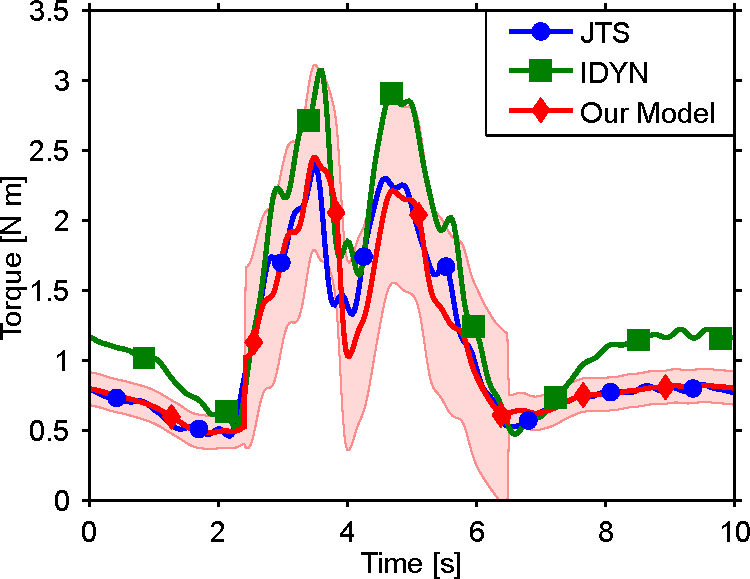
\includegraphics[width=.99\hsize]{robertoICRA/fig/exp2_model}
% 		\caption{\textbf{\nameref{sec:results:exp2}}: Prediction for the \textcolor{red}{medium contact} on the joint \textit{shoulder 2} (for visualization purposes JTS and \idyn{} are filtered).
% 		Even if a contact in this position was not observed during learning, the single contact model was robust to small variations in the position of the obstacle.}
% 		\label{fig:exp2:model_contact}
% 		\end{minipage}
% 	\end{figure}
% 	%
	
	%
	\begin{figure}[t]
		\resizebox{\hsize}{!}{
		\centering
		\begin{subfigure}[t]{0.48\hsize}
			\centering
			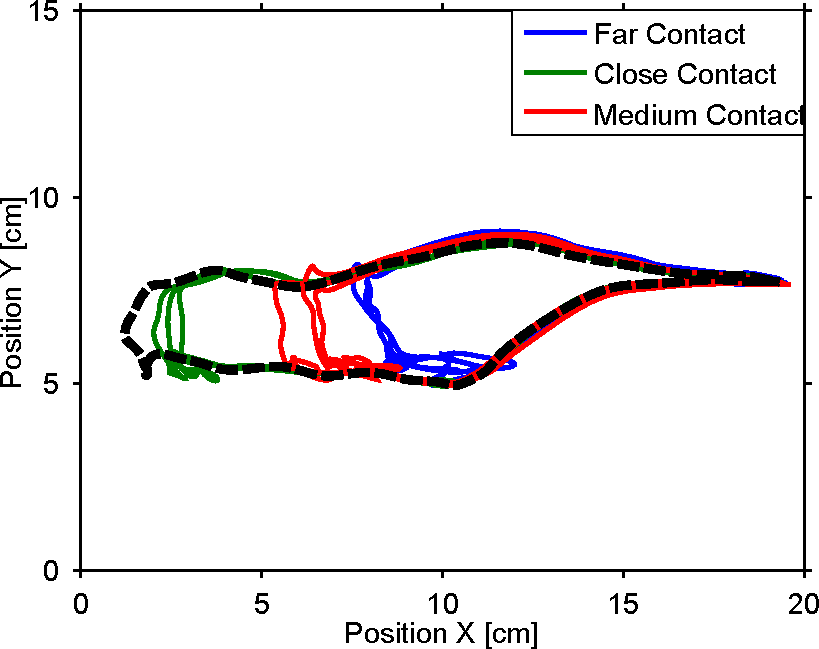
\includegraphics[height=4.2cm]{robertoICRA/fig/generalized_contact_a.pdf} %[width=.99\columnwidth]
			\caption{Task space}
			\label{fig:effects_contact:a}
		\end{subfigure}
		\hfill
		\begin{subfigure}[t]{0.48\hsize}
			\centering
			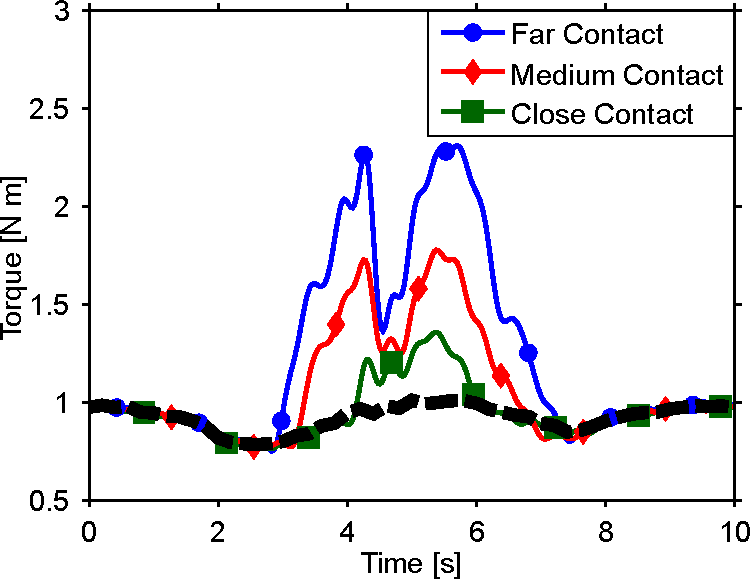
\includegraphics[height=4.2cm]{robertoICRA/fig/generalized_contact_b.pdf} % [width=.99\columnwidth]
			\caption{Torque}
			\label{fig:effects_contact:b}
		\end{subfigure}
		}
		\caption{\textbf{\nameref{sec:results:exp2}:} Effects of the contact on the task space and the torque for the three different contact types: contact 1 (far), contact 2 (medium) and contact 3 (close). 
		The task in absence of contact is displayed as reference (\textbf{black dashed curve}). 
		%\comment{Figures generated by \textit{Figures\_exp2}}
		}
		\label{fig:exp2:effects_contact}
        \figspace
	\end{figure}
	%
	
	
%\todo{say about no gating network}
	%We now extend the single contact experiment to cover generalized single contacts.\todo{what is a generalized contact?}
	In the following, we show that the prediction performance of each GP expert is robust to small variations in the position of the contact.
	This is important since the exact position of the obstacle does not need to be known in advance (within a single expert $f_j$).
	As in the previous experiment we consider a tracking task along a circular trajectory.
	However, this time the obstacle is placed at one of three different positions along the trajectory: close, medium and far.
    Each of these obstacles is shifted 2\,cm along the horizontal axis.
	Obstacles at different positions along the trajectory lead to different effects in terms of both joint position and torque signal, as clearly visible in~\fig\ref{fig:exp2:effects_contact}.
	Note that the skin input~$\skinInput$ will also be affected, as shown in~\fig\ref{fig:exp2:skin}. 
    Hence, we could potentially learn a separate expert for each contact. 
    However, we only consider a single expert as we want to demonstrate the robustness of a single expert, not of the gating network.
	%Therefore, we assume that the gating network has been appropriately devised to consider the three different contacts as belonging to the same family of contacts, rather than three different contacts.
    
    %
	\begin{figure}[t]
		\centering
		\begin{subfigure}[t]{0.30\hsize}
        \centering
			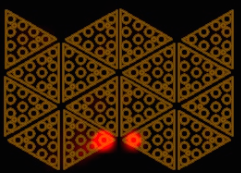
\includegraphics[height=1.8cm]{robertoICRA/fig/paris2_new} 
			\caption{Contact 1}
		\end{subfigure}
		\hspace{0.1cm}
		\begin{subfigure}[t]{0.30\hsize}
        \centering
			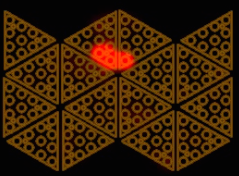
\includegraphics[height=1.8cm]{robertoICRA/fig/paris3_new} 
			\caption{Contact 2}
		\end{subfigure}
		\hspace{0.1cm}
		\begin{subfigure}[t]{0.30\hsize}
        \centering
			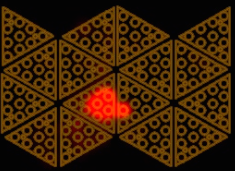
\includegraphics[height=1.8cm]{robertoICRA/fig/paris7_new}
			\caption{Contact 3}
		\end{subfigure}
		\caption{\textbf{\nameref{sec:results:exp2}}. The different contact locations detected by the forearm skin respectively for the three contacts: contact~1 (far), contact~2 (medium) and contact~3 (close).}
		\label{fig:exp2:skin}
        \figspace
	\end{figure}
	%

	% 
	\begin{table}[t]
		\resizebox{\hsize}{!}{
		\centering
		\begin{tabular}{|l|l|c|c|c|}
			\hline 
			& Method	& Shoulder 1 [Nm] & Shoulder 2 [Nm] & Elbow [Nm] \\
			\hline 	
			\multirow{2}{*}{Far contact}  & \idyn 	& $0.13 \pm 3.9 \times 10^{-3}$  &  $0.40 \pm 9.7\times 10^{-3}$ & $0.06 \pm 1.9\times 10^{-3}$ \\ 
			&Our model 		& $\mathbf{0.06  \pm 1.9\times 10^{-3}}$ & $\mathbf{0.08  \pm 2.9\times 10^{-3}}$ & $\mathbf{0.03  \pm 8.0 \times 10^{-4}}$\\
			\hline 	
			\multirow{2}{*}{Close contact}  & \idyn 	& $0.09 \pm 2.2\times 10^{-3}$ & $0.22 \pm 4.5\times 10^{-3}$ & $0.04 \pm  0.9\times 10^{-3}$\\ 
			&Our model 		& $\mathbf{0.06  \pm 1.4\times 10^{-3}}$ & $\mathbf{0.06 \pm 1.4\times 10^{-3}}$ & $\mathbf{0.02  \pm 6.3\times 10^{-4}}$ \\ % 0.58 0.58 is correct!
			\hline 	
			\multirow{2}{*}{Medium contact}  & \idyn 	& $0.10 \pm 2.8\times 10^{-3}$ & $0.32 \pm 6.7\times 10^{-3}$ & $0.05 \pm 1.3\times 10^{-3}$ \\ 
			&Our model 		& $\mathbf{0.06 \pm 1.7\times 10^{-3}}$ & $\mathbf{0.12 \pm 4.7\times 10^{-3}}$ & $0.05 \pm 1.7\times 10^{-3}$ \\
			\hline
		\end{tabular}
		}
		\caption{\textbf{\nameref{sec:results:exp2}:} Errors between the ground truth~(JTS) and the predictions with either the \idyn{} and our learned model on the test set. 
		A single expert is robust to small variations of the contact.
		}
		\label{tab:exp2}
        \figspace
	\end{table}
	%
    
    %\todo[inline]{Not sure what the experiment was doing that you described above. The notion of the gating network just appeared at the end.}
	%The contact model is learned using the data collected at 40 Hz from contact 1 and contact 3 (far and close contacts), summing up to a total of 978 data points.
    The contact model is learned using the data collected from contact 1 and contact 3 (far and close contacts) and as validation the data set generated from the \textit{unseen} contact 2 (medium) is used.
	%\comment{Describe dataset: 978 datapoints, 40 Hz}
	%We learn a model using the collected data from two of the obstacles (close and far), and test the resulting model on the third (medium) \textit{unseen} obstacle.
	In \tab\ref{tab:exp2}, the RMSE for all three contacts are reported for \idyn{} and our learned model, respectively.
	The results show that the learned model is robust to unseen contacts and performs  equally well or better than the analytic model \idyn{}. 
	%\fig\ref{fig:exp2:model_contact} shows an example of the prediction for the unseen contact.



%===============================================================================


\subsection{Learning multiple contacts}
\label{sec:results:exp3}


   
% 	%
% 	\begin{figure}[t]
% 		\centering
% 		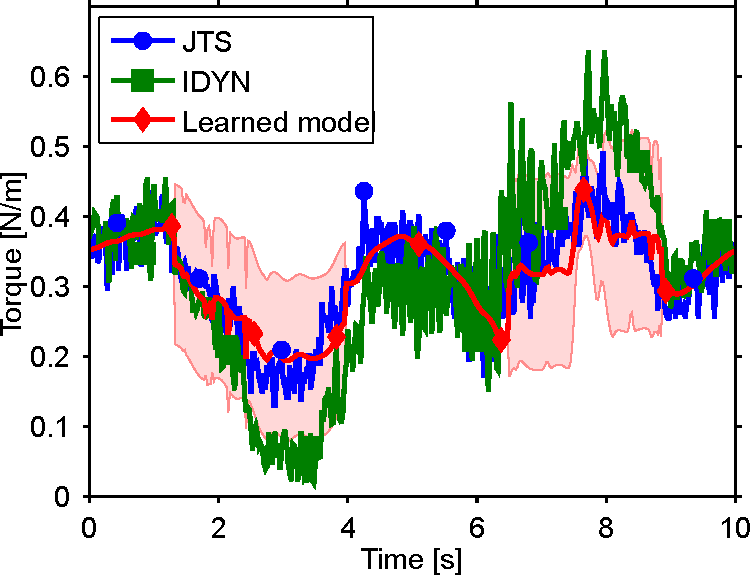
\includegraphics[width=.60\linewidth]{robertoICRA/fig/exp3_1}\\
% 		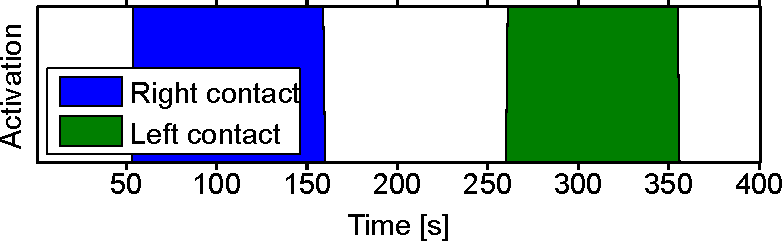
\includegraphics[width=.60\linewidth]{robertoICRA/fig/exp3_2}
% 		\caption{\textbf{\nameref{sec:results:exp3}:} Prediction of torques in presence of multiple contacts. 
% 		Various models are shown, but individually, none of them correctly capture the dynamics of the system. 
% 		Our approach combine them to successfully generalize to unseen configurations.
% 		}
% 		\label{fig:exp3:gating}
% 	\end{figure}
% 	%
		% 
	\begin{table}[t]
		\resizebox{\hsize}{!}{
		\centering
		\begin{tabular}{|l|l|c|c|c|}
			\hline 
			& Method	& Shoulder 1 [Nm] & Shoulder 2 [Nm] & Elbow [Nm] \\
			\hline 	
			\multirow{2}{*}{Right contact} & \idyn{} & $0.10\pm 1.3 \times 10^{-3}$ & $0.13\pm 1.6 \times 10^{-3}$ & $0.06\pm 8.1 \times 10^{-4}$ \\ 
			& Our model 		& $\mathbf{0.04\pm 6.3 \times 10^{-4}}$ & $\mathbf{0.07\pm 1.2 \times 10^{-3}}$ & $\mathbf{0.02\pm 2.7 \times 10^{-4}}$ \\
			\hline
			\multirow{2}{*}{Left contact}  & \idyn{} & $0.08 \pm 1.2 \times 10^{-3}$ & $0.16 \pm 2.0 \times 10^{-3}$ & $0.05 \pm 8.2 \times 10^{-4}$ \\ 
			& Our model 		& $\mathbf{0.03 \pm 5.7 \times 10^{-4}}$ & $\mathbf{0.07 \pm 9.6 \times 10^{-4}}$ & $\mathbf{0.02 \pm 2.8 \times 10^{-4}}$ \\
			\hline
			\multirow{2}{*}{Both contacts}  & \idyn{} & $0.10 \pm 1.3 \times 10^{-3}$ & $0.11 \pm 1.4 \times 10^{-3}$ & $0.07 \pm 8.4 \times 10^{-4}$ \\ 
			& Our model 		& $\mathbf{0.05\pm 8.3 \times 10^{-4}}$ & $\mathbf{0.10\pm 1.6 \times 10^{-3}}$ & $\mathbf{0.03 \pm 4.0 \times 10^{-4}}$ \\
			\hline
		\end{tabular}
		}
		\caption{\textbf{\nameref{sec:results:exp3}:} Root mean square error between the ground truth~(JTS) and the predictions with the \idyn{} and our learned model on the test set. 
		Our learned model predicts the torque more accurately than \idyn{}.
		}
		\label{tab:exp3}
        \figspace
	\end{table}
	%
	%
    After learning single contacts, we now show how to combine the learned models to adapt to unseen and more complex environments with multiple contacts.
	We consider a scenario having the \robot{} performing a circular motion with its left arm.
	%We initially generate a reference trajectory without any obstacle.
	We initially performed two experiments with an obstacle either on the left and on the right of the reference trajectory (see \fig\ref{fig:exp3:icuparis_experiment_bars}).
	%These obstacles clearly limit the motion of the end effector as shown in \fig\ref{fig:exp3:effects_contacts_pos:a} and \fig\ref{fig:exp3:effects_contacts_pos:b}.
	With the data collected in these two contact cases, we trained two independent expert models $f_1$, $f_2$, one for each contact.
	We repeated the experiment, but this time with both left and right contacts 
    %(see \fig\ref{fig:exp3:effects_contacts_pos:a}) 
    and used this last unseen case to validate our models. 
\fig\ref{fig:exp3:gating} shows an example of the prediction and the corresponding activation of the two contact models. 
	During both the right and the left contact, the corresponding experts are activated by the gating network.
	Therefore, we can successfully combine the contributions of the single contact models learned to generalize to unseen cases with multiple contacts.
	 \tab\ref{tab:exp3} reports the RMSE for the predictions.
     We notice that even in this experiment the experts accurately learn the effects of single contacts.
     Moreover, the gating network allows us to combine the experts to generalize to unseen environments, such as in the case of both contacts. 
     

%  	%
% 	\begin{figure}[t]
% 		\centering
% 		\begin{subfigure}[t]{0.32\hsize}
% 			\centering
% 			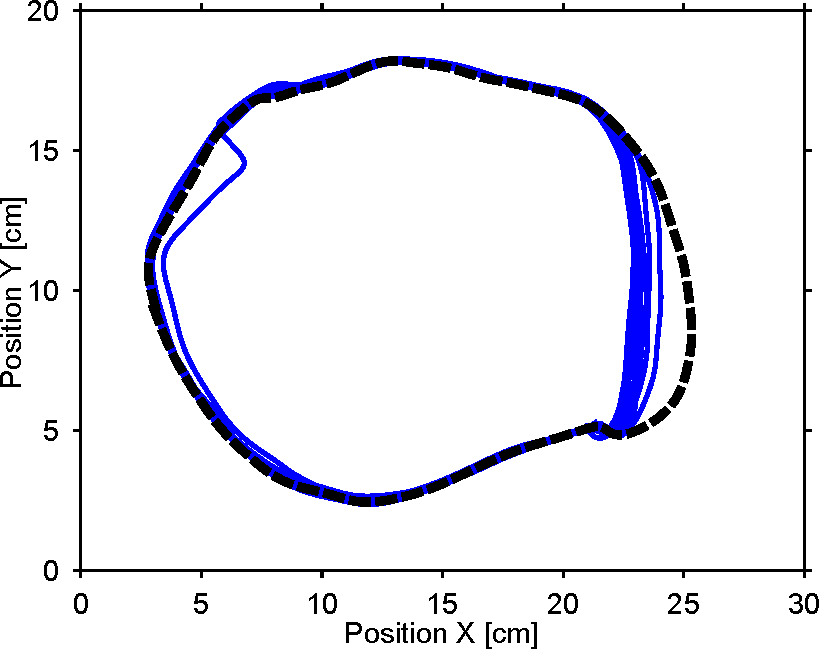
\includegraphics[width=.99\columnwidth]{robertoICRA/fig/Double_contact_a}
% 			\caption{Right contact}
% 			\label{fig:exp3:effects_contacts_pos:a}
% 		\end{subfigure}
% 		\hfill
% 		\begin{subfigure}[t]{0.32\hsize}
% 			\centering
% 			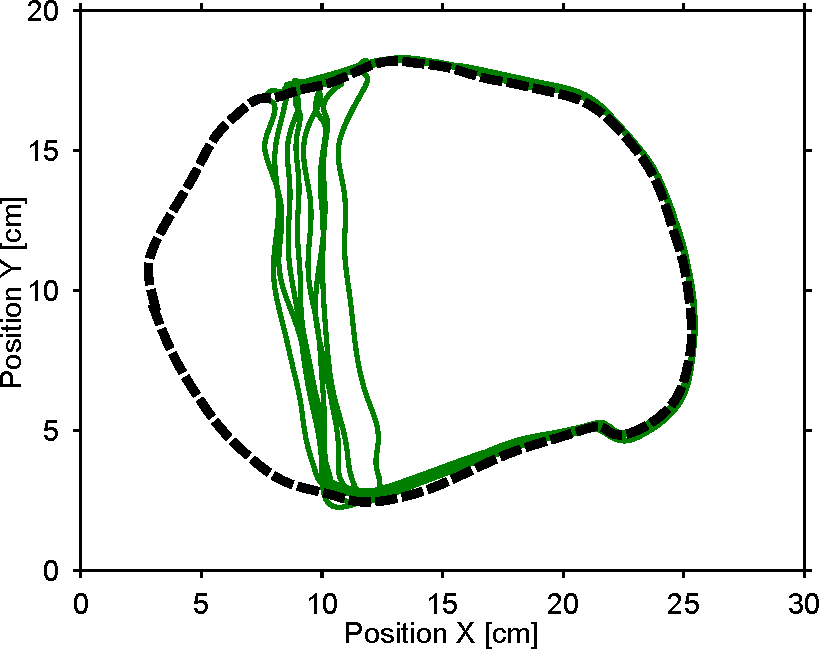
\includegraphics[width=.99\columnwidth]{robertoICRA/fig/Double_contact_b}
% 			\caption{Left contact}
% 			\label{fig:exp3:effects_contacts_pos:b}
% 		\end{subfigure}
% 		\hfill
% 		\begin{subfigure}[t]{0.32\hsize}
% 			\centering
% 			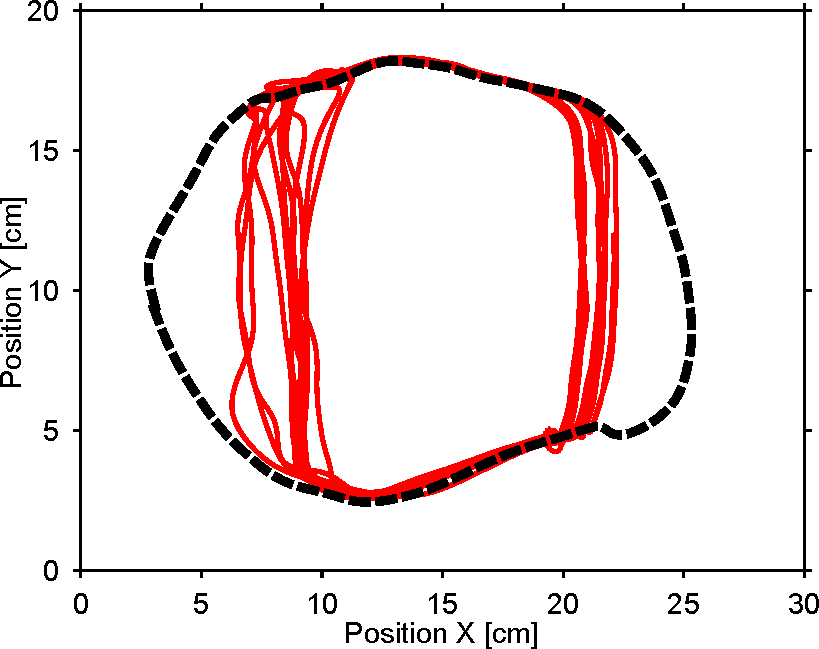
\includegraphics[width=.99\columnwidth]{robertoICRA/fig/Double_contact_c}
% 			\caption{Both contacts}
% 			\label{fig:exp3:effects_contacts_pos:c}
% 		\end{subfigure}
% 		\caption{\textbf{\nameref{sec:results:exp3}:} Effect of contacts in the task space for the three different case of contacts - \textcolor{blue}{right contact}, \textcolor{darkgreen}{left contact} and \textcolor{red}{both left and right contacts}. 
% 		The task in absence of contact is displayed as reference (\textbf{black dashed curve}). 
% 		%\comment{Figure generated by \textit{SomeFigures}}
% 		}
% 		\label{fig:exp3:effects_contacts_pos}
% 	\end{figure}
% 	%
 %

	%\begin{wrapfigure}{r}{0.46\columnwidth}
	\begin{figure}[t]
		\begin{minipage}{.32\linewidth}
			\centering
			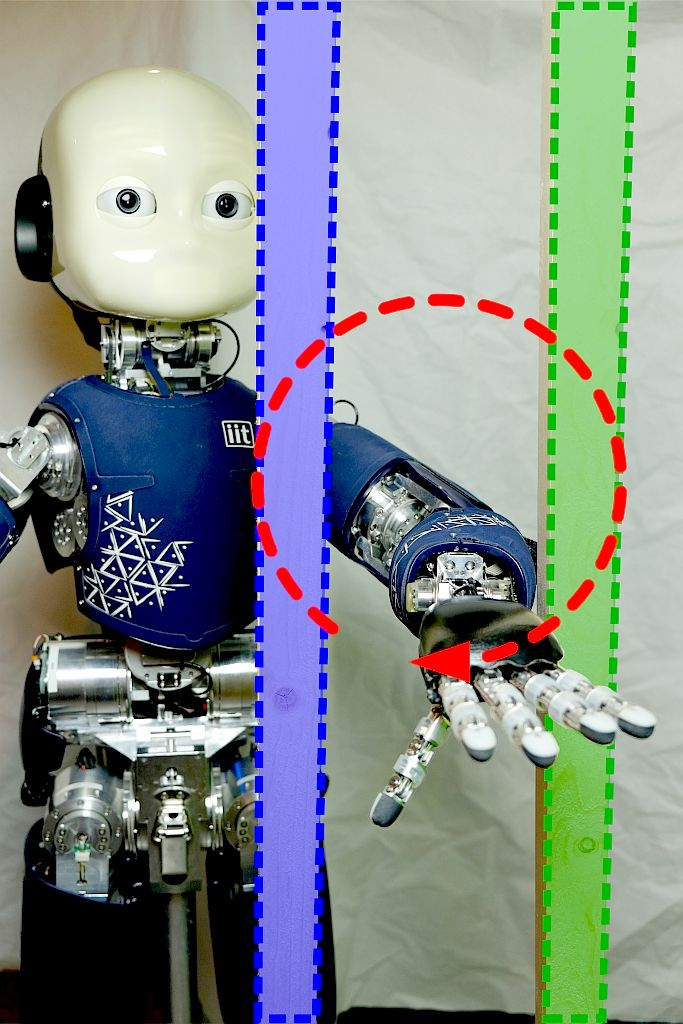
\includegraphics[width =.99\linewidth]{robertoICRA/fig/iCubParis02_Double_Contact}
			\caption{\textbf{\nameref{sec:results:exp3}:} The robot performs a circle with its left arm. 
			The forearm collides alternatively with the left, the right or both contacts.}
			\label{fig:exp3:icuparis_experiment_bars}
		\end{minipage}	
		\hfill
		\begin{minipage}{.52\linewidth}
			\centering
			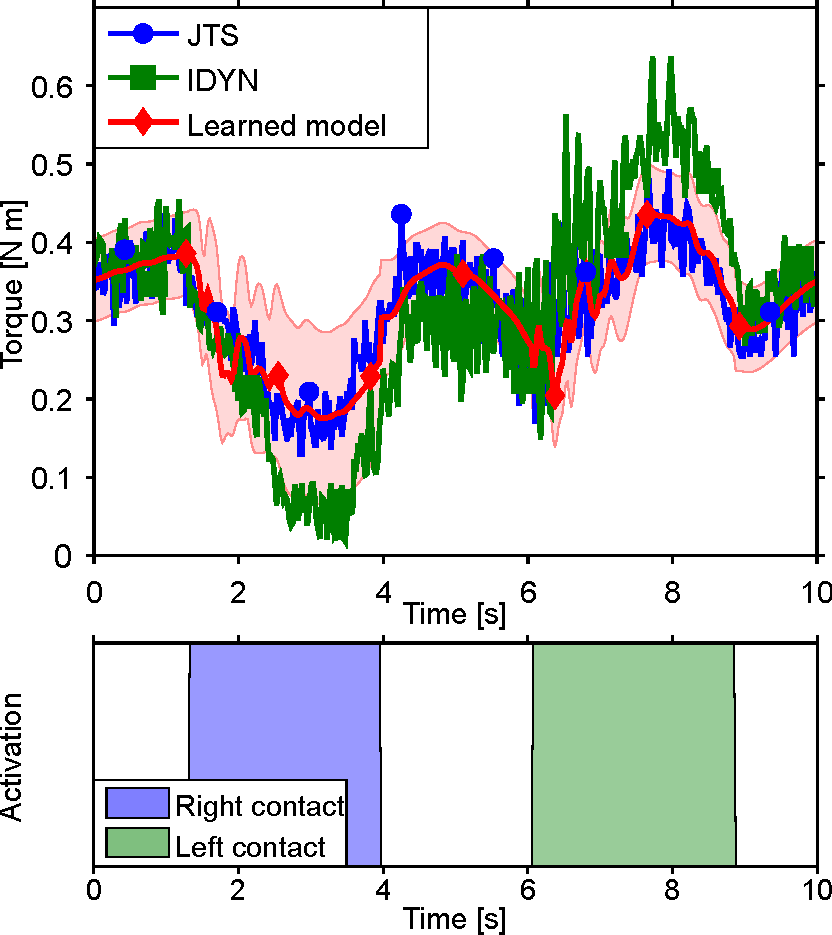
\includegraphics[width=.99\linewidth]{robertoICRA/fig/exp3_both}
			\caption{\textbf{\nameref{sec:results:exp3}:} Prediction of torques with multiple contacts and the corresponding activation of the gating network.
			%Various models are shown, but individually, none of them correctly capture the dynamics of the system. 
			Our mixture-of-experts model combines single-contact models to a multiple-contact model.
			}
			\label{fig:exp3:gating}
		\end{minipage}	
        \figspace
	\end{figure}
	%\end{wrapfigure}
	%


%===============================================================================

\subsection{Learning the gating network}
\label{sec:results:exp5}

	%An important component of our model is the gating network, which activates the different experts~$f_j$.
    %\todo[inline]{This is the first time I'm reading about experts...}
	So far, we assumed a heuristic gating network to select the active experts.
	%However, with growing complexity of the number and types of contacts, also the complexity of the gating network increases.
	%Hence, it will be valuable to automatically learn the gating network, which is equivalent to learning a classifier, which detects and recognizes the various types of contacts.
	In this experiment we show that a learned gating network achieves a comparable accuracy as a manually devised heuristic.
    As ground truth to evaluate the performances, as well as for training the classifier, we labeled the data with one of the following labels: no contact, left contact, right contact.
    The heuristic is based on thresholds of the activation of the skin input~$\skinInput$ and the force torque sensors~$\ftsForces$.
	We train a Support Vector Machine (SVM) classifier (using the library LIBSVM~\cite{Chang2011}) having as input $\q, \skinInput, \ftsForces$ and as output the contact labels (none, left, right).

	We evaluated the performance of the trained classifier on an unseen test set.
	\fig\ref{fig:exp5:accuracy} shows that the learned SVM achieved a classification accuracy that is similar to the heuristic gating network. 
    Equivalent results are obtained in terms of RMSE of the inverse dynamics when comparing the experts models learned by the gating networks.
    %A similar result is indicated in terms of RMSE when using the experts models based on the gating networks (see \tab\ref{tab:exp5b}).
    However, training the gating network (i.e., training the SVM classifier) requires considerably less expert knowledge compared to designing a heuristic. 
    As there is no visible performance difference, we conclude that training the gating network is generally preferable.
Increasing the number of training data may further increase the accuracy of the gating network.




% 	% 
% 	\begin{table}[t]
% 		\resizebox{\hsize}{!}{
% 		\centering
% 		\begin{tabular}{|l|c|c|c|}
% 			\hline 
% 			Gating network	& No Contact & Contact 1 & Contact 2 \\
% 			\hline 	
% 			Heuristic		&		\%	& x\% & x\% \\ 
%               Learned 		& 94.2 \%   		& 89.1 \% & 75.9 \% \\ 
% 			\hline
% 		\end{tabular}
% 		}
%  		\caption{\textbf{\nameref{sec:results:exp5}:} Classification accuracy for the heuristic gating network and the learned one using SVM.}
% 		\label{tab:exp5a}
% 	\end{table}
% 	%
% 	% 
% 	\begin{table}[t]
% 		\resizebox{\hsize}{!}{
% 		\centering
% 		\begin{tabular}{|l|c|c|c|}
% 			\hline 
% 			Gating network	& Shoulder 1 [Nm] & Shoulder 2 [Nm] & Elbow [Nm] \\
% 			\hline 	
% 			Learned (SVM)& $0.057 \pm 9.72\times 10^{-4}$ & $0.140 \pm 4.36\times 10^{-3}$ & $0.033 \pm 5.42\times 10^{-4}$\\ 
% 			Heuristic 		& $0.057  \pm 5.42\times 10^{-4}$ & $0.140  \pm 3.74\times 10^{-4}$ & $0.034 \pm 5.72\times 10^{-4}$\\ 
% 			\hline
% 		\end{tabular}
% 		}
% 		\caption{\textbf{\nameref{sec:results:exp5}:} Comparison of the RMSE when using the heuristic gating network and the learned one using SVM.}
% 		\label{tab:exp5b}
% 	\end{table}
% 	% 

%%%%%%%%%%%%%%%%%%%%%%%%%%%%%%%%%%%%%%%%%%%%%%%%%%%%%%%%%%%%%%%%%%%%%%%%%%%%%%%%%

\section{Conclusions}
\label{sec:conclusion}

	%\comment{A conclusion section is not required. Although a conclusion may review the main points of the paper, do not replicate the abstract as the conclusion. A conclusion might elaborate on the importance of the work or suggest applications and extensions.}


%The main contribution of this paper is a technique to learn the inverse dynamics model of robots under the effect of multiple and simultaneous contacts exerted on the whole robot structure. 
%In whole-body robot control, estimating contact forces accurately is crucial
%may not only be understood as nuisance that need to be avoided. Making contacts may rather be seen as a desirable feature 
%for balance and stabilization, and to increase the number of potential actions that the robot is able to execute, e.g., reach for distant objects.
%, to stabilize or even . 
Whole-body control strategies that exploit contacts need accurate models of the system dynamics.
%to be stable and precise. 
This is crucial for balance and stabilization, and to increase the number of potential actions that the robot is able to execute, e.g., creating a contact to reach for distant objects.
%
We introduced a data-driven mixture-of-experts approach based on Gaussian processes  for learning inverse dynamics models with contacts. 
% A  was proposed to deal with multiple contacts. %model these non-linear effects. 
We evaluated our model on the \robot{} humanoid robot using tactile sensors and force/torque sensors as model inputs.  
We showed that the model accurately predicts contact forces and outperforms a state-of-the-art analytical approach used to estimate the joint torques in \robot{}. 
The estimation from the learned model does not rely on dynamic parameters, but it is completely data-driven and based on tactile sensors and force/torque sensors. %to determine the amount of external forces.
As a result, our approach does not require a spatially calibrated model of the skin~\cite{DelPrete2011,DelPrete2012}.
% Neither spatially calibrated models of the skin~\cite{DelPrete2011,DelPrete2012} nor preceise knowledge about the contact location were required --- in contrast to the analytical modeling strategy. 
This is a promising feature for robust control strategies that explicitly takes contacts into account. 
%In future, we will incorporate our inverse dynamics models in active control tasks involving multiple contacts in whole-body structure, such as balancing with multiple supports in rigid and compliant environments.

% In future work, we will incorporate our inverse dynamics models in active control tasks using rewards as training signals to overcome the need of labels or ground truth data.

%, which involve multiple simultaneous contacts.
%and as such we could utilize the mixing property of the experts.

% Our solution enables a fast and accurate prediction of the joint torques in situations when the robot is in contact (or not) with an object, detected by a tactile skin.
% The estimation from the learned model does not rely on dynamic parameters, but it is completely data-driven by using tactile sensors and force/torque sensors to determine the amount of external forces.
% As a result, our approach does not requires a spatially calibrated model of the skin~\cite{DelPrete2011,DelPrete2012}.
% With the increasing availability of larger arrays of skin sensors, this kind of data-driven approach greatly reduces the design/engineering complexity.
% %
% %It only introduces an additional sensor measurement $\skinInput$, which provides the information about the contact location and a measure of the applied force on the taxels. 
% Moreover, tactile sensors are cheaper and lighter than joint torque sensors. 
% With our approach, it is possible to apply torque control to robotic manipulators even with contacts at locations other than the end-effector, which makes it possible to control the robot while physically interacting with an evolving environment or humans.

% \todo[inline]{kill this paragraph?\\
% Another advantage of our data-driven approach is that model predictive control needs rapid computation, since it has to compute the entire robot dynamics over a receding time horizon at each control step (as in \cite{naveau2014metapod}, within 1--2~$\mu$s).
% The use of a learned model such as GP potentially allows to reduce the computational time at prediction time and hence to be beneficially used in fast real time applications.}

	%
	\begin{figure}[t]
			\centering
			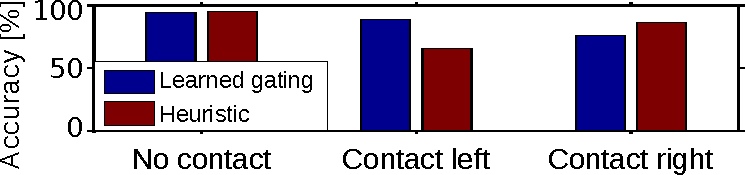
\includegraphics[width=.94\hsize]{fig/exp5_accuracy_red}
		\caption{\textbf{\nameref{sec:results:exp5}:} Classification accuracy for the heuristic and learned SVM gating networks.
		}
		\label{fig:exp5:accuracy}
        \figspace
	\end{figure}
	% 

%\addtolength{\textheight}{-12cm}   % This command serves to balance the column lengths
                                  % on the last page of the document manually. It shortens
                                  % the textheight of the last page by a suitable amount.
                                  % This command does not take effect until the next page
                                  % so it should come on the page before the last. Make
                                  % sure that you do not shorten the textheight too much.

%%%%%%%%%%%%%%%%%%%%%%%%%%%%%%%%%%%%%%%%%%%%%%%%%%%%%%%%%%%%%%%%%%%%%%%%%%%%%%%%


%%%%%%%%%%%%%%%%%%%%%%%%%%%%%%%%%%%%%%%%%%%%%%%%%%%%%%%%%%%%%%%%%%%%%%%%%%%%%%%%

%\section*{APPENDIX}

%Appendixes should appear before the acknowledgment.


%%%%%%%%%%%%%%%%%%%%%%%%%%%%%%%%%%%%%%%%%%%%%%%%%%%%%%%%%%%%%%%%%%%%%%%%%%%%%%%%

%% Sere: to save some space
%\section*{Acknowledgments}
%
%We thank Vincent Padois and Alain Droniou for their help with \textit{iCubParis02}.
%\medskip
%\noindent
%\textit{Acknowledgments}: 
%\section*{Acknowledgments}
%We thank Vincent Padois and Alain Droniou for their help with \textit{iCubParis02}.

%the iCub facility of the Italian Institute of Technology (IIT) for the technical support provided, and 
%Vincent Padois and Alain Droniou for their help with iCubParis02.
%\fixme{We also thank Vincent \& Alan from UPMC}
 
%
%The research leading to these results has received funding from the European Community's Seventh Framework Programme (FP7/2007--2013) under grant agreements \#270327 (CompLACS) and \#600716 (CoDyCo) and the Department of Computing, Imperial College London.
% The preferred spelling of the word ÒacknowledgmentÓ in America is without an ÒeÓ after the ÒgÓ. Avoid the stilted expression, ÒOne of us (R. B. G.) thanks . . .Ó  Instead, try ÒR. B. G. thanksÓ. Put sponsor acknowledgments in the unnumbered footnote on the first page.


%%%%%%%%%%%%%%%%%%%%%%%%%%%%%%%%%%%%%%%%%%%%%%%%%%%%%%%%%%%%%%%%%%%%%%%%%%%%%%%%

%\clearpage

\bibliographystyle{abbrv}
\bibliography{ICRA2015}



\end{document}